\documentclass[12pt,spanish,Letterpaper,openany]{book}
\usepackage{lmodern}
\usepackage{setspace}
\setstretch{0.85}
\usepackage{amssymb,amsmath}
\usepackage{ifxetex,ifluatex}
\usepackage{fixltx2e} % provides \textsubscript
\ifnum 0\ifxetex 1\fi\ifluatex 1\fi=0 % if pdftex
  \usepackage[T1]{fontenc}
  \usepackage[utf8]{inputenc}
\else % if luatex or xelatex
  \ifxetex
    \usepackage{mathspec}
  \else
    \usepackage{fontspec}
  \fi
  \defaultfontfeatures{Ligatures=TeX,Scale=MatchLowercase}
    \setmainfont[Scale=1.0, HyphenChar=None]{Corbel}
    \setsansfont[]{Corbel}
    \setmonofont[Mapping=tex-ansi]{Corbel}
\fi

\makeatletter
\renewcommand\mainmatter{\clearpage\@mainmattertrue\pagenumbering{arabic}}
\renewcommand\frontmatter{\clearpage\@mainmatterfalse\pagenumbering{arabic}}
\renewcommand\backmatter{\clearpage\@mainmatterfalse}
\makeatother

%\usepackage{etoolbox}
%\makeatletter
%\patchcmd{\@smemmain}{\cleardoublepage}{\clearpage}{}{}
%\patchcmd{\@smemmain}{\cleardoublepage}{\clearpage}{}{}
%\patchcmd{\@smemfront}{\cleardoublepage}{\clearpage}{}{}
%\patchcmd{\@smemfront}{\cleardoublepage}{\clearpage}{}{}
%\makeatother

\setlength{\parindent}{0em}

\usepackage{graphicx}
\usepackage{booktabs}
\usepackage{multicol}
\usepackage{doc}
\usepackage{float}
\usepackage{tcolorbox} 
\usepackage{lipsum}
\usepackage{tikz}
\usepackage{nonfloat}

\usepackage{pdfpages}

\usepackage[
contents={},
opacity=1,
scale=1.5,
color=blue!90
]{background}
\usepackage{lipsum}
\usepackage{ifthen}

\usepackage{xcolor}
\usepackage[pagestyles]{titlesec}

\renewpagestyle{plain}[\normalsize\sffamily\bfseries\slshape]{
  \setfoot{}{\color{white}{\thepage}}{}}

\newpagestyle{myps}[\normalsize\sffamily\bfseries\slshape]{
  \setfoot{}{\color{white}{\thepage}}{}}
  
\pagestyle{myps}


\usepackage{framed}
\definecolor{colorlinetitle}{HTML}{a87e00}%{a87e00}%
\definecolor{textlinetitle}{HTML}{061769}%{061769}%{061769}%
\definecolor{fondo}{HTML}{041d57}%
\definecolor{newfondo}{HTML}{3d0718}%
\colorlet{shadecolor}{fondo!81!}


% use upquote if available, for straight quotes in verbatim environments
\IfFileExists{upquote.sty}{\usepackage{upquote}}{}
% use microtype if available
\IfFileExists{microtype.sty}{%
\usepackage{microtype}
\UseMicrotypeSet[protrusion]{basicmath} % disable protrusion for tt fonts
}{}
\usepackage[inner=12.7mm,outer=12.7mm,top=25mm,bottom=21.0mm]{geometry}
\usepackage{hyperref}
\hypersetup{unicode=true,
            pdftitle={Revista de la Unidad de Prácticas de Ingeniería y EPS},
            pdfauthor={Unidad de Prácticas de Ingeniería y EPS},
            pdfborder={0 0 0},
            breaklinks=true}
\urlstyle{same}  % don't use monospace font for urls
\ifnum 0\ifxetex 1\fi\ifluatex 1\fi=0 % if pdftex
  \usepackage[shorthands=off,main=spanish]{babel}
\else
  \usepackage{polyglossia}
  \setmainlanguage[]{spanish}
\fi
\usepackage{natbib}
\bibliographystyle{apalike}
\usepackage{longtable,booktabs}
\IfFileExists{parskip.sty}{%
\usepackage{parskip}
}{% else
\setlength{\parindent}{0pt}
\setlength{\parskip}{6pt plus 2pt minus 1pt}
}
\setlength{\emergencystretch}{3em}  % prevent overfull lines
\providecommand{\tightlist}{%
  \setlength{\itemsep}{0pt}\setlength{\parskip}{0pt}}
\setcounter{secnumdepth}{5}
% Redefines (sub)paragraphs to behave more like sections
\ifx\paragraph\undefined\else
\let\oldparagraph\paragraph
\renewcommand{\paragraph}[1]{\oldparagraph{#1}\mbox{}}
\fi
\ifx\subparagraph\undefined\else
\let\oldsubparagraph\subparagraph
\renewcommand{\subparagraph}[1]{\oldsubparagraph{#1}\mbox{}}
\fi

%%% Use protect on footnotes to avoid problems with footnotes in titles
\let\rmarkdownfootnote\footnote%
\def\footnote{\protect\rmarkdownfootnote}


  \title{Revista de la Unidad de Prácticas de Ingeniería y EPS}
    \author{Unidad de Prácticas de Ingeniería y EPS}
      \date{2021-10-27}

% no title page
\AtBeginDocument{\let\maketitle\relax}

\usepackage{caption}
\captionsetup{%
labelsep=colon,%
font={footnotesize},%
aboveskip=0.5\baselineskip,%
belowskip=0\baselineskip,% deve essere 0 perché regolo lo spazio dal testo con \intextsep
}%


\usepackage{booktabs}
\usepackage{longtable}

\usepackage{indentfirst}
\setlength{\parindent}{1em}
\usepackage{enumitem}
\setlist[itemize]{labelindent = \parindent, leftmargin=*}

%\usepackage{framed,color}
%\definecolor{shadecolor}{RGB}{248,248,248}

\renewcommand{\textfraction}{0.05}
\renewcommand{\topfraction}{0.8}
\renewcommand{\bottomfraction}{0.8}
\renewcommand{\floatpagefraction}{0.75}

\renewcommand{\chaptername}{Artículo}
\addto\captionsspanish{\renewcommand{\chaptername}{Artículo}}
\addto\captionsspanish{\renewcommand{\contentsname}{Índice General}}


\frenchspacing
\tolerance=5000
\multicoltolerance=3000 

\raggedbottom
\raggedcolumns

\setlength{\columnsep}{1em}
%We want a rule between columns.
%\setlength\columnseprule{.4pt}

%Tambien queremos asegurarnos de que un nuevo entorno multicols 
%encuentre suficiente espacio en la parte inferior de la pagina.
\setlength\premulticols{6\baselineskip}

%Al equilibrar columnas, ignoramos las soluciones que son 
%demasiado malas. Ademas, si la ultima columna es demasiado mala, 
%la tipeamos sin estirar.
\setcounter{columnbadness}{7000}
\setcounter{finalcolumnbadness}{7000}

\newcommand{\prefacetitlecommand}%
{\titleformat{\chapter}[display]%
{\bfseries\large\color{colorlinetitle}}%
{\relax}%
{0ex}%
{{\titlerule[1.2pt]}\filright\color{textlinetitle}}[\color{colorlinetitle}\vspace{0.5ex}{\titlerule[1.2pt]}]%
}


\newcommand{\articletitlecommand}%
{\titleformat{\chapter}[display]%
{\bfseries\Large\centering\color{colorlinetitle}}%
{\relax}%
{0ex}%
{{\titlerule[1.2pt]}\filright\color{textlinetitle}}[\color{colorlinetitle}\vspace{0.5ex}{\titlerule[1.2pt]}]%
}



\newcommand{\sectionCenter}%
{\titleformat{\section}[block]%
{\bfseries\large\color{textlinetitle}\filcenter}%
{\relax}%
{0ex}%
{\empty}%
}


\newcommand{\sectionRight}%
{\titleformat{\section}[block]%
{\bfseries\large\color{textlinetitle}}%
{\relax}%
{0ex}%
{\empty}%
}


\newcommand{\subsectionRight}%
{\titleformat{\subsection}[block]%
{\bfseries\normalsize\color{textlinetitle}}%
{\relax}%
{0ex}%
{\empty}%
}

\usepackage{titletoc}
\titlecontents{chapter}[3em]
{\vspace{5mm}}
{\normalsize\contentslabel[\color{textlinetitle}\thecontentslabel]{2em}\color{black}\itshape\normalsize}
{\color{black}\itshape\normalsize}
{\color{colorlinetitle}\titlerule*[.3pc]{.}\color{black}\contentspage}

\newcommand{\tcolorboxcommand}{\begin{tcolorbox}[sharp corners=uphill, colback=newfondo, colframe=newfondo, arc=6mm, boxrule=0mm, boxsep=0mm]}

\newcommand{\photocommand}[2]{%
\fcolorbox[HTML]{DCEEA7}{DCEEA7}{%
\begin{minipage}{95.19mm}%
	\hspace{1mm}%
	\begin{minipage}{22.49mm}%
		\vspace{1mm}%
		\includegraphics[width=22.49mm, height=31.96mm]{#1}%
		\vspace{1mm}%
	\end{minipage}%
	\hspace{2.4mm}%
	\begin{minipage}{68.80mm}%
		#2
	\end{minipage}%
	\hspace{0.5mm}%
\end{minipage}%
}%
}

\definecolor{fondobiography}{HTML}{DCEEA7}

\NewDocumentEnvironment{photobiography}{m O{}}%
{%
\begin{tcolorbox}[colback=fondobiography, colframe=fondobiography, width=97.19mm, boxsep=-2mm, arc=0mm]
\begin{minipage}{95.19mm}%
	%\hspace{1mm}%
	\begin{minipage}{22.49mm}%
		\vspace{2mm}%
		\includegraphics[width=22.49mm, height=31.96mm]{#1}%
		\vspace{2mm}%
	\end{minipage}%
	\hspace{2.4mm}%
	\begin{minipage}{68.80mm}%
	#2%
}%
{%
	\end{minipage}%
	%\hspace{0.5mm}%
\end{minipage}%
\end{tcolorbox}
}


\newcommand{\spacetext}{\vspace{8.1mm}}
\newcommand{\minimalspacetext}{\vspace{1mm}}
\newcommand{\spaceelevenmilis}{\vspace{11mm}}
\newcommand{\spacetenmilis}{\vspace{10mm}}
\newcommand{\spaceninemilis}{\vspace{9mm}}
\newcommand{\spaceeightmilis}{\vspace{8mm}}
\newcommand{\spacesevenmilis}{\vspace{7mm}}
\newcommand{\spacesixmilis}{\vspace{6mm}}
\newcommand{\spacefivemilis}{\vspace{5mm}}
\newcommand{\spacefourmilis}{\vspace{4mm}}
\newcommand{\spacethreemilis}{\vspace{3mm}}
\newcommand{\spacetwomilis}{\vspace{2mm}}
\newcommand{\spaceinitialeditorialcontenido}{\vspace{8.1mm}}
\newcommand{\spaceoneminus}{\vspace{-1mm}}
\newcommand{\spacetwominus}{\vspace{-2mm}}
\newcommand{\spacefourminus}{\vspace{-4mm}}
\newcommand{\hideFromPandoc}[1]{#1}
\hideFromPandoc{ \let\Begin\begin \let\End\end }
\newcommand{\minipagepartone}{\begin{minipage}[c]{3cm}}
\newcommand{\minipagetwocolumn}{\noindent\begin{minipage}[c]{\columnwidth}}
\newcommand{\minipageparttwo}{\end{minipage}\begin{minipage}[c]{12cm}}
\newcommand{\minipageparttwochapter}{\end{minipage}\begin{minipage}[c]{15cm}}
\newcommand{\minipageendpart}{\end{minipage}}
\newcommand{\firstparteditorial}{\begin{longtable}[]{@{}ll@{}}\endhead\begin{minipage}[t]{0.47\columnwidth}\raggedright}
\newcommand{\firstparttwoeditorial}{\begin{longtable}[l]{@{}ll@{}}\endhead\begin{minipage}[t]{0.47\columnwidth}\raggedright}
\newcommand{\midleparteditorial}{\end{minipage} & \begin{minipage}[t]{0.47\columnwidth}\raggedright}
\newcommand{\lastparteditorial}{\end{minipage}\end{longtable}}

\newcommand{\HRule}{\begin{center}\rule{0.5\linewidth}{0.2mm}\end{center}}

\begin{document}
\maketitle

% \pagestyle{plain}
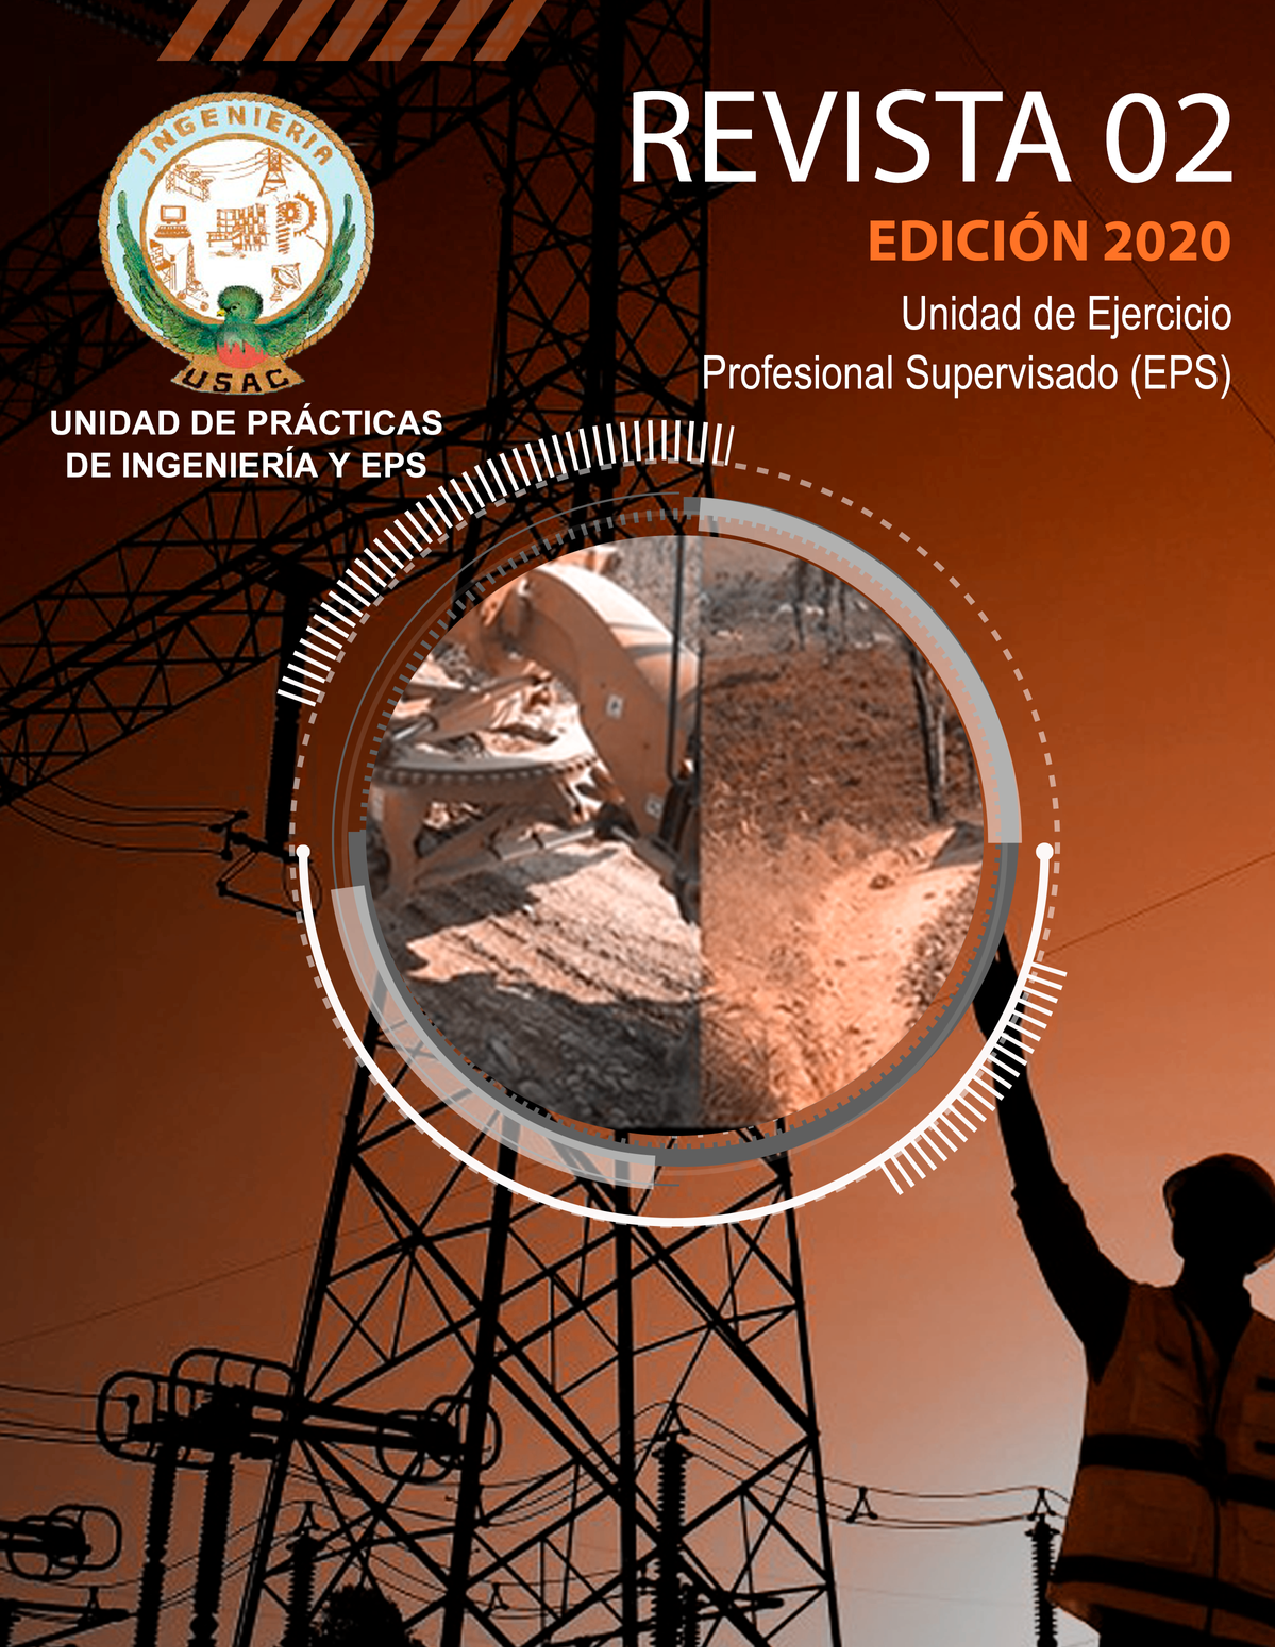
\includepdf{images/cover.pdf}

\AddEverypageHook{%
\ifthenelse{\value{page}<44}%
{\ifthenelse{\isodd{\value{page}}}%
  	{\backgroundsetup{scale=1, color=white, opacity=1, angle=0, contents={
\includegraphics[width=\paperwidth,height=\paperheight]{latex/background_numberimpar.pdf}}}}%
  	{\backgroundsetup{scale=1, color=white, opacity=1, angle=0, contents={
\includegraphics[width=\paperwidth,height=\paperheight]{latex/background_numberpar.pdf}}}}%
}{}%
\BgMaterial}

%%%%%%{
%%%%%%\setcounter{tocdepth}{0}
%%%\tableofcontents
%%%}
%%%%%%%%%%%%\listoffigures
%%%
\prefacetitlecommand

\titlespacing*{\chapter} {0pt}{0pt}{2pt}

\titleformat{\chapter}[display]
{\normalfont\color{black} \bfseries}
{\empty}
{0pt}
{\filcenter\Huge}

\begin{center}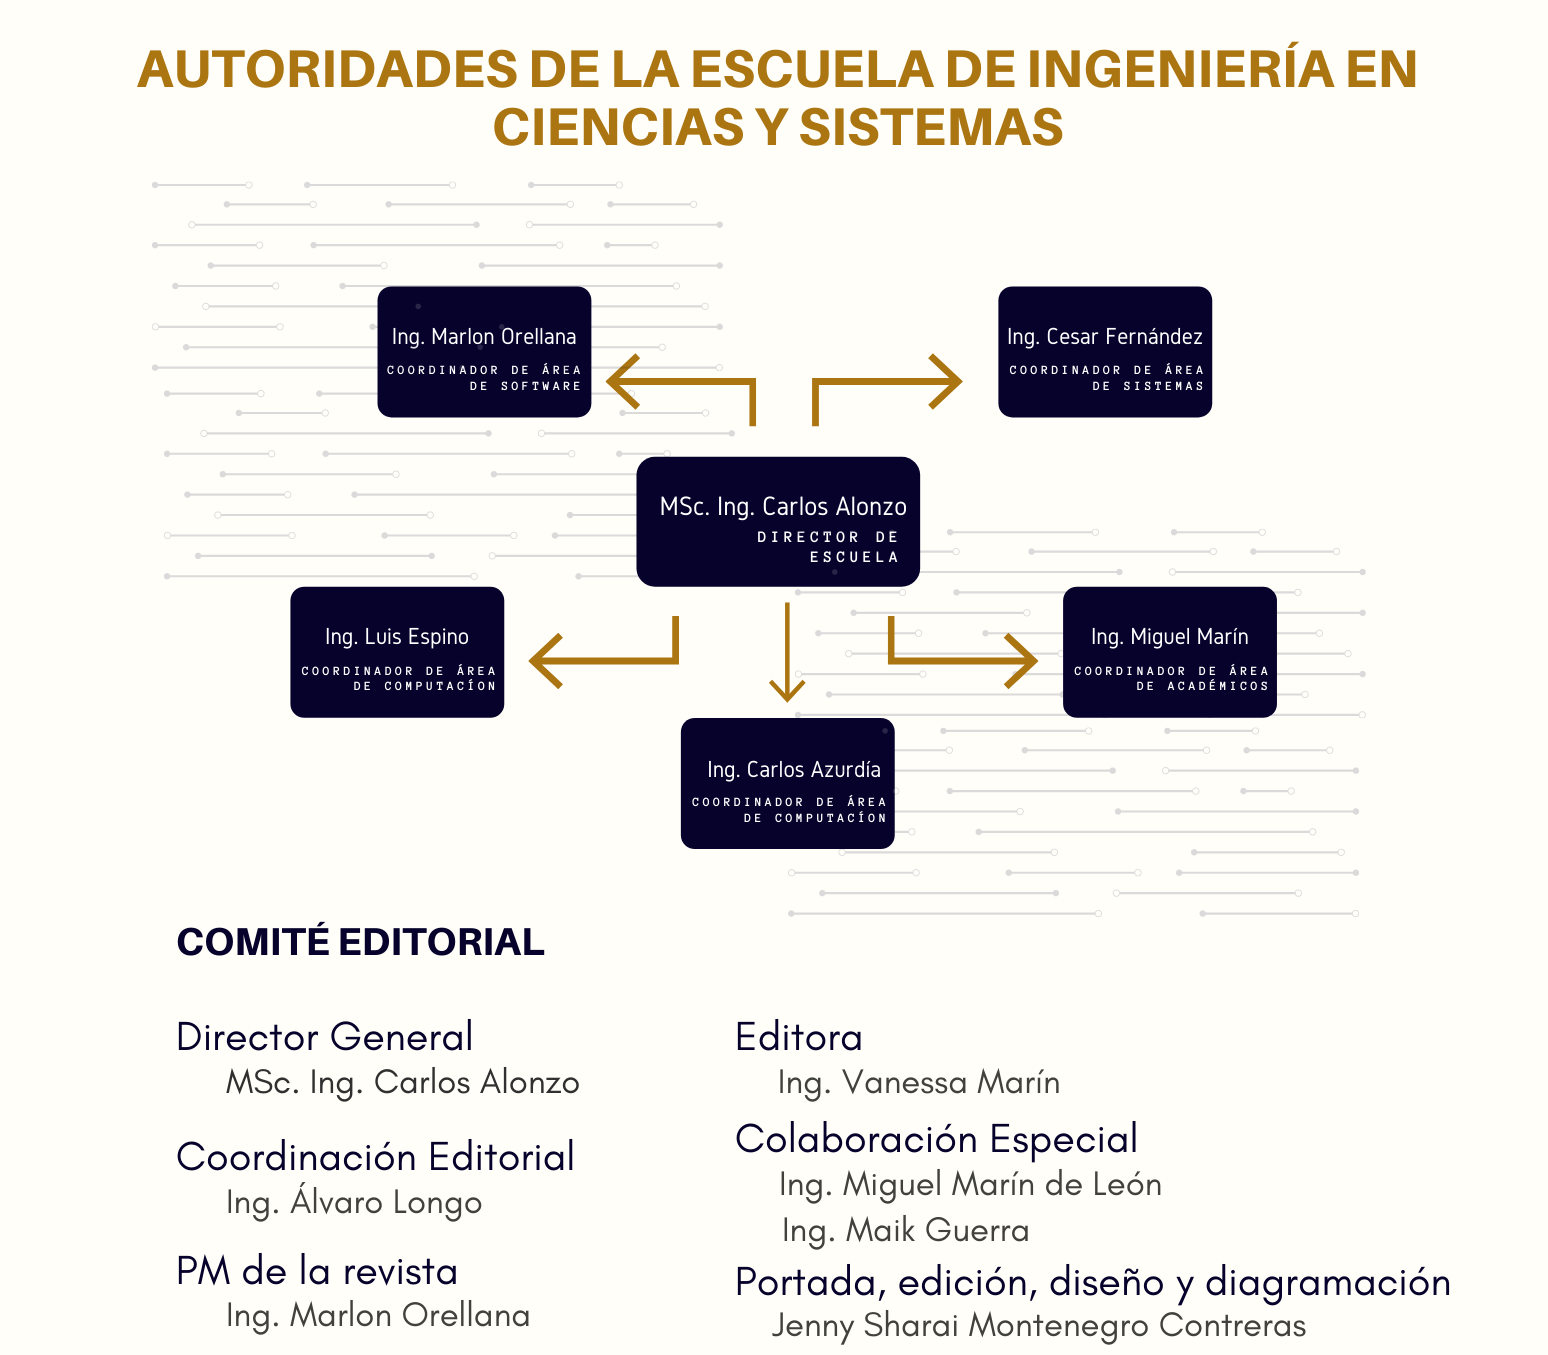
\includegraphics[width=1\linewidth]{images/organigrama} \end{center}

\hypertarget{editorial}{%
\chapter*{Editorial}\label{editorial}}
\addcontentsline{toc}{chapter}{Editorial}

El área de tecnología se hace cada vez más presente en cada una de las disciplinas de la ciencia y en la cotidianidad de la vida, su presencia ha permitido distintos avances en múltiples áreas. Es así como hoy en día se plantean nuevos retos para los profesionales en las áreas de tecnología, los cuales requieren mantener una gama mucho más amplia de conocimiento y de aplicación. Lo cual demanda su versatilidad y capacidad para entender ``el negocio'' con una mayor agilidad a la vez de tener la capacidad de innovar en éste.

Es así como cada vez se abre paso a un ritmo mucho mas vertiginosos disciplinas como el internet de las Cosas IoT, o inteligencia artificial. La primera permite tener una presencia casi omnipresente, relacionando múltiples elementos y tecnologías con el fin de crear soluciones que cada vez se masifican más.

Por otro lado, el desarrollo en el campo de la inteligencia artificial, ha permitido aumentar la capacidad de procesamiento y respuesta, cambiando la lógica del trabajo y ocupación humana, en la cual no es la excepción el área de tecnología, que también se ha visto remplazada en la realización de sus propias tareas, principiando por las de carácter más mecánico. Pero a la vez ha aperturando nuevos nichos. Haciendo cada vez más accesible tecnología y herramientas, las cuales permitirán el desarrollo e irradiación de la presencia de profesionales de sistemas.

Pero el reto no solo va en función del conocimiento, también demanda un balance ético en su proceder, así como una claridad de dirección, toda vez que parte de su perfil demandará características de liderazgo cada vez más.

\setcounter{tocdepth}{0}
\tableofcontents

\articletitlecommand

\titlespacing*{\chapter} {0pt}{-20pt}{4pt}

\hypertarget{pareja46}{%
\chapter{Análisis de mortalidad vs vacunación}\label{pareja46}}

\begin{center}
\includegraphics[width=1\linewidth]{images/pareja46_01} \end{center}

\begin {multicols}{2}

\hypertarget{introducciuxf3n}{%
\section{Introducción}\label{introducciuxf3n}}

En el año 1796 Edwar Jenner se sorprendió que granjeros de su localidad contraían viruela
vacuna y que al superar la enfermad ya no contraían la variante humana al estar en exposición
con enfermos. Realizo un experimento, inoculo a un niño con líquido de la postula de un
enfermo con la variante vacuna, el niño desarrollo la enfermedad de manera leve; pero el
decidió intentarlo una nueva vez, pero en esta ocasión con la variante humana, el resultado
fue inesperado, el niño no desarrollo la enfermedad. Este descubrimiento permitió erradicar
la viruela en el año 1979 por la OMS.

Hoy en día las vacunas han salvado a 2.5 millones de personas cada año según la organización
de la salud, pero también 2 millones de personas fallecen por falta de acceso a las vacunas
existentes. Pero hoy en día existen otro problema, existen grupos de personas a través de
redes sociales llamados ``antivacunas'', este grupo inculca miedo y generar dudas sobre las
personas a tal grado que deciden no participar en jornadas de vacunación.

La vacunación tiene muchos beneficios, pues además de prevenir enfermedades hoy en día
también permite disminuir la mortalidad y el riesgo de sufrir secuelas a causa de
enfermedades mortales como poliomielitis y actualmente Coronavirus.

\hypertarget{artuxedculo}{%
\section{Artículo}\label{artuxedculo}}

\textbf{¿Como Lograr Campañas Exitosas de Vacunación contra COVID 19?}

Muchos países en Latinoamérica se están planteando la meta de logar la inmunización de
entre el 60\% al 80\% de la población. Esto con el fin que la efectividad de las vacunas que se
encuentran actualmente disponibles puedan detener la propagación y/o mutación de la
enfermedad.

El éxito para lograr este objetivo es garantizar una amplia cobertura de la población que
puede vacunarse, así como campañas masivas que den a conocer los beneficios de las
vacunas. Un desafió es la población de mayor edad, pues este grupo no tiene acceso en
muchos casos a medios electrónicos donde poder informarse sobre los lugares donde pueden
vacunarse, horarios de atención, disponibilidad de dosis, etc.

Una forma en que se puede medir que tan efectivas son las campañas de vacunación, es
cuantificar la cantidad de programas que existen previos a la pandemia y analizar la cobertura
que tienen estas campañas. Estas campañas permiten identificar patrones sobre limitaciones
culturales, geográficas, económicas, entre otras. Actualmente según La Organización para la
Cooperación y el Desarrollo Económicos (OCDE) el 87\% de la población tiene acceso a
poder inmunizarse, sin embargo, las autoridades de cada país son las encargadas de poder
garantizar que ese porcentaje de cobertura se cumpla o por el contrario el porcentaje
disminuya.

\textbf{¿Como la tecnología puede ayudar a las campañas de vacunación?}

Hoy en día las tecnologías actuales son un arma para poder inmunizar más personas, así como
poder dar información a la población sobre los acontecimientos que suceden en su región.
Empresas como Facebook implementaron cambios en sus políticas, las cuales, exponen son
en favor de proteger a las personas contra la información no verídica o que transmite datos
antivacunación, incluso sus restricciones para empresas que deseen anunciar productos de
higiene contra el virus y mascarillas sanitarias, pues deben tener como mínimo cuatro meses
de haber ingresado como anunciantes a Facebook y quedan terminante prohibido anuncios
masivos pues la explotación de estos productos puede ser utilizado como medio de
acaparamiento y explotación de otras personas. Queda prohibido la venta de vacunas contra
el COVID-19 o pruebas conta el COVID-19 pues estos intentos de ventas no generan tácticas
de ayuda a la población sino de explotación y de beneficiar a un grupo selecto de personas.
Las tácticas de terror así como los anuncios que ofrecen protección total o eliminación del
virus queda totalmente prohibidas.

\textbf{¿Como la tecnología puede ayudar en el desarrollo de vacunas?}

Actualmente se busca explotar la inteligencia artificial como arma para respaldar tareas como
la fabricación y distribución de vacunas. Tras el inicio de la pandemia y el desarrollo de
vacunas en tiempo récord, se encontró el reto de fabricarlas, distribuirlas y administrarlas.

La comunidad de personas que se dedica al campo de la inteligencia artificial encontró una
posición para poder apoyar los esfuerzos del desarrollo o reutilización de tecnologías que
permitieran tomar mejores decisiones. La Inteligencia artificial puede ayudar con los
siguientes problemas:

\begin{itemize}
\item
  \textbf{Reducir incertidumbre:} La inteligencia artificial no elimina la incertidumbre sino por
  el contrario ayuda a reducirla. Un ejemplo es que los científicos utilizaron modelos
  de datos de propagación del virus COVID--19 para predecir la propagación de la
  enfermedad con mayor precisión. Los modelos creados se han distribuido entre las
  comunidades médicas y científicas para poder crear modelos de distribución y
  administración de vacunas, esto para poder disponer de las vacunas en las áreas donde
  la propagación del virus es más alta y así tener disposición de datos sobre la eficiencia
  de la vacuna y mejorar los pronósticos de los modelos de propagación.
\item
  \textbf{Generar modelos sobre tareas repetitivas:} La fabricación, distribución y
  administración de las vacunas a gran escala es una tarea tediosa, pero estas tareas son
  muchas veces se toman decisiones comerciales o económicas, como la gestión de
  pedidos y la clasificación de los pacientes que la recibirán. La inteligencia artificial
  puede trabajar 24 horas y 7 días a la semana, esto es una ventaja porque su juicio
  también es en pro de que se logre la mayor cobertura y disminuir la cantidad de
  contagios, al contrario de una persona que puede afectar su juicio por temas culturales
  o socioeconómicos.
\item
  \textbf{Ayudar a determinar las personas que deben recibir vacuna:} Determinar que personas
  de la población y en qué orden debe ser, son preguntas desafiantes y que muchas
  veces debe ser el ser humano quien deba decidir, pues son vidas las que están juego,
  sin embargo, la Inteligencia Artificial puede optimizar o apoyar las decisiones
  complejas, pues garantiza la equidad e identificar los grupos de población que deben
  priorizarse pues ya sea que están en primera fila combatiendo el virus o porque bien
  tienen razones para rechazarla y generar más contagios.
\end{itemize}

Otro ejemplo de la inteligencia artificial ayudando a problemas existentes, es el mapeo y
visualización de la red de suministros, la visibilidad del inventario y la previsión de adquirir
mayor stock de vacunas. Sin embargo, cada región, país o institución tiene desafíos propios
ya sea por limitación de recursos tecnológicos o por que se cree que la inteligencia artificial
desplaza al ser humano por máquinas que harán un mejor trabajo y por ende las personas
sean más bien un simple peón en esta lucha conta el COVID-19.

\textbf{Problemas durante la vacunación en Guatemala}

En Guatemala, el proceso de vacunación contra el COVID-19 se ha llevado a cabo de forma alarmante-
mente lenta. Comenzando con la adquisición de las vacunas a los distintos
proveedores o a través del método COVAX y con la aplicación a la población. Fue hasta
finales de enero cuando se aprobó el decreto 1-2021 que aprobaba el presupuesto y el
mecanismo para realizar compras directas de las vacunas.

El gobierno había presentado desde finales del 2020 el Plan Nacional de Vacunación, que se
dividía en cuatro fases, que abarcaban a distintos sectores de la población. El propósito con
este plan era el de priorizar a los distintos sectores, según el riesgo de contagio que tienen
desde sus actividades o por enfermedades.

Siguiendo el modo de inscripción que aplicaron otros países como México, el ministerio de
salud habilitó un sitio web (\url{https://registrovacunacovid.mspas.gob.gt/}) para el registro de las
personas que quisieran vacunarse. El registro se hace ingresando el código personal de
identificación DPI.

Para poder realizar el registro, el sistema debe validar que la persona cumple con ser parte
del grupo de personas que abarca la fase actual ya que, si no se cumple con esa restricción,
el sistema rechaza la inscripción. Una característica que aseguraba el sistema es que luego de
realizar el registro, se le comunicaría a la persona a través de mensaje de texto al teléfono
registrado la fecha, hora y lugar a donde debe llegar para vacunarse.

Desde antes de tener el primer lote de vacunas, el gobierno habilitó el sitio web para que las
personas que entran en la primera fase pudieran inscribirse. El primer problema que tuvo el
sistema es que la alta demanda de acceso al sitio web, provocó la caída del servidor. Esto
provocó muchas críticas al sistema ya que las personas debían esperar hasta horas para poder
inscribirse.

Al comenzar la vacunación de la primera fase, el sitio web mantuvo un funcionamiento
considerablemente estable, las personas se registraban y después de unos días recibían el
mensaje con los datos de su cita de vacunación. Ocurrió también un problema con la
recepción de los datos de la cita, ya que por falta de comunicación o de instrucciones claras,
muchas personas registraban números de casa y desde esos dispositivos no es posible recibir
mensajes de texto.

\hypertarget{conclusiones}{%
\section{Conclusiones}\label{conclusiones}}

\begin{itemize}
\item
  Desde el inicio, el sitio web lanzado por el MSPAS ha sufrido bastantes problemas
  que pueden deberse a la mala planificación y diseño o también por los constantes
  cambios a las restricciones debido a la falta de coherencia desde el gobierno central
  a las fases del Plan Nacional de Vacunación.
\item
  Empresas tecnológicas están sumándose al esfuerzo por ayudar a que la información
  de las vacunas llegue a todos los grupos que tienen acceso, así como permitir que se
  distribuya y agilicen estos datos que permitan la vacunación de estos grupos.
\item
  Tecnologías como la inteligencia artificial, pueden jugar un rol importante en el
  proceso de tomas de decisiones de la vacunación, así como la optimización de los
  recursos para poder llegar a todos los sectores de la población
\end{itemize}

\hypertarget{referencias}{%
\section{Referencias}\label{referencias}}

\begin{itemize}
\item
  {[}1{]} \href{https://www.caf.com}{Pena, Federico.} (15 de enero 2021). \href{https://www.usac.edu.gt/}{USAC:} \href{https://www.caf.com/es/conocimiento/visiones/2021/01/como-lograr-campanas-exitosas-de-vacunacion-contra-el-covid19-en-america-latina/}{\emph{¿Cómo lograr campañas exitosas de vacunación contra el COVID-19 en América Latina?}}. Recuperado de: \url{https://bit.ly/3ueCUt2}. {[}Último acceso: agosto de 2021{]}.
\item
  {[}2{]} \href{http://www.repositorio.usac.edu.gt/}{Facebook for business.} (1 de enero 2021).\href{https://www.facebook.com/business/help/1123969894625935}{\emph{Adver- tising Policies Related to Coronavirus (COVID-19)}}. Recuperado de: \url{https://bit.ly/2Zz99YT}. {[}Último acceso: agosto de 2021{]}.
\item
  {[}3{]} \href{https://www.whatsapp.com}{Centro de información sobre coronavirus de Whatsapp.} (1 de enero 2021). \href{https://www.whatsapp.com/coronavirus/?lang=es}{\emph{Cómo puede ayudarte WhatsApp a estar conectado durante la pandemia de coronavirus (COVID-19)}}. Recuperado de: \url{https://bit.ly/2Wcx7Yy}. {[}Último acceso: agosto de 2021{]}.
\item
  {[}4{]} \href{https://www.bbvaopenmind.com}{Barral, Miguel.} (12 de julio 2021). \href{https://www.bbvaopenmind.com/ciencia/apuntes-cientificos/tecnologias\%02nueva-revolucion-en-vacunas/}{\emph{Cuatro tecnologías para una nueva revolución en vacunas \textbar{} OpenMind}}. Recuperado de: \url{https://bit.ly/3ubCK5T}. {[}Último acceso: agosto de 2021{]}.
\item
  {[}5{]} \href{https://health.economictimes.indiatimes.com}{Sicular, Svetlana.} (31 de marzo 2021). \href{https://health.economictimes.indiatimes.com/news/health-it/4-ways-ai-can-help-with-covid-19-vaccination-svetlana-sicular/81782358}{\emph{4 Ways AI Can Help With Covid-19 Vaccination: Svetlana Sicular - ET HealthWorld}}. Recuperado de: \url{https://bit.ly/3COyKey}. {[}Último acceso: agosto de 2021{]}.
\item
  {[}6{]} \href{http://www.repositorio.usac.edu.gt/4300/}{Who Team.} (28 de octubre 2020). \href{https://www.who.int/es/news-room/q-a-detail/coronavirus-disease-(covid-19)-vaccines?adgroupsurvey=\%7Badgroupsurvey\%7D\&gclid=Cj0KCQjwpreJBhDvA}{\emph{Enfermedad por el coronavirus (COVID-19): Vacunas}}. Recuperado de: \url{https://bit.ly/39BHsR1}. {[}Último acceso: mayo de 2020{]}.
\item
  {[}7{]} \href{http://www.repositorio.usac.edu.gt/4300/}{Montenegro, Sofía.} (26 de abril 2021). \href{https://dialogos.org.gt/blog/tropiezos-en-el-proceso-de-vacunacion-contra-la-covid-19-en-guatemala}{\emph{Tropiezos en el proceso de vacunación contra la COVID-19 en Guatemala}}. Recuperado de: \url{https://bit.ly/3lYZjHf}. {[}Último acceso: agosto de 2021{]}.
\end{itemize}

\end {multicols}

\medskip

\HRule

\medskip

\hypertarget{pareja52}{%
\chapter{La tecnología como una parte fundamental para la logística en la distribucíon de vacunas contra COVID-19}\label{pareja52}}

\begin{center}
\includegraphics[width=1\linewidth]{images/pareja52_02} \end{center}

\begin {multicols}{2}

El mundo al fin ve una salida a la crisis generada por el COVID-19; los procesos para obtener
una cura en un lapso de tiempo sin precedentes en la historia. Varias farmacéuticas iniciaron
estudios, ensayos, y procesos para la creación y producción de sus vacunas, aunque las
fórmulas desarrolladas no son 100\% efectivas; permiten disminuir la tasa de mortalidad y
lograr que las restricciones impuestas por varios gobiernos se levanten, encaminando así la
sociedad a la normalidad que alguna vez tuvimos.

La distribución de las vacunas desde un inicio sufre varios problemas; desde la compra
desmesurada de varios países, hasta la aplicación de dosis en los pacientes; esto último
implica otros obstáculos a los gobiernos relacionados a la logística en la distribución; como
coordinar medios de transporte para los cargamentos de vacunas, brindar acceso de la vacuna
a toda la población, conservar las fórmulas a una temperatura determinada, movilizar estas
dosis a poblados remotos, crear un plan para priorizar a un sector de la población para la
aplicación y la habilitación de centros adecuados para los pacientes.

Junto a los esfuerzos y el trabajo de varias instituciones se implementan varias soluciones
tecnológicas que apoyan a la distribución y aplicación de las vacunas a la población.

\begin{itemize}
\tightlist
\item
  \textbf{SAP's Vaccine Collaboration Hub (VCH)}
\end{itemize}

Como primer paso para una distribución equitativa de las vacunas, se deben identificar a las
poblaciones más vulnerables. Para lograr que la vacuna llegué a todas partes cuanto antes, los
gobiernos y las farmacéuticas deben estar sincronizados; es por ello que surge una plataforma
desarrollada por SAP. Se trata del Centro de Colaboración de Vacunas de SAP (Vaccine
Collaboration Hub, VCH), es una herramienta que acompaña a los gobiernos del mundo a
llevar un proceso de distribución de las vacunas desde su inicio y todo lo que conlleva, hasta
el fin exitoso.

Esta innovadora plataforma consta de tres valiosas capas. La primera, es la que se encarga de
dar transparencia en la visibilidad y seguimiento de las vacunas, para mitigar aquellos errores
que conlleven a las interrupciones, así como controlar las fechas de caducidad de los lotes de
vacunas. Como segunda capa, se encuentran las soluciones para tener la máxima eficacia en
administración y así predecir la demanda de medicamentos. Y como última instancia, el
software permite capturar y responder a las métricas de operaciones en tiempo real y con esto
percibir la respuesta de la población ante el proceso de vacunación.

\begin{itemize}
\tightlist
\item
  \textbf{Sistemas de Información Geográfica (GIS)}
\end{itemize}

Estos sistemas permiten asociar una serie de datos a una localización geográfica. Esto quiere
decir que los distintos sistemas de salud pueden identificar instalaciones capaces de
almacenar y distribuir la vacuna, identificar y priorizar poblaciones críticas, identificar
brechas en el acceso y formular opciones de distribución alternativas, implementar un sistema
de gestión e inventario de vacunas, brindar transparencia y comunicación precisa a través de
paneles que se estarán actualizando en tiempo real.

\emph{``La tecnología GIS se ha utilizado durante mucho tiempo para varios tipos de selección de
sitios y es especialmente útil cuando se consideran criterios complejos, como accesibilidad,
composición de la población, ingreso y egreso, presupuesto y más''}.Al desarrollar
herramientas con sistemas GIS países como Estados Unidos pueden reaccionar y desarrollar
planes distintos dependiendo de lugares que se pueden identificar fácilmente al mantener
actualizados y enriquecidos los mapas que se diseñaron.

\begin {flushleft}
\noindent\begin{minipage}[c]{\columnwidth}


\includegraphics[width=1\linewidth]{images/pareja52_01}
\figcaption{Situación de COVID-19 en Guatemala, Ministerio de Salud Pública y Asistencia Social,
actualiza 30 de agosto 2021.}

\end{minipage}

\end {flushleft}

\textbf{Sitios en línea para registrar cita para vacunación}

Las dosis fabricadas por las farmacéuticas no son suficientes para la demanda actual, por lo
que en varios países se implementaron planes para la priorización de sectores que recibirán
antes la vacuna, algunas veces agrupando por fases a los distintos sectores y planificando
citas en varios puestos oficiales para la aplicación, como la mayoría de soluciones requieren
más de una dosis, estas etapas también serán manejadas por estos sistemas y podrán ser
consultadas por los pacientes.

Para llevar el control en varios países se crean portales web que a través de la cooperación de
varias instituciones gubernamentales permiten al público por medio de un documento de
identificación registrarse y agendar una cita para la aplicación de la dosis. Estos sistemas
pueden validar si la persona cumple con los criterios de la fase activa y por medio de la
dirección seleccionada o registrada se programara una cita en la ubicación más próxima.

Confiar en una plataforma de tecnología permite actualmente hacer un poco más manejable la
situación para los gobiernos o entidades de salud involucradas. Generar planes de
distribución, pensar en sistemas de distribución, comunicarse con la población, manejarse con
claridad y gran transparencia en los procesos; permite conocer el estado actual del COVID-19
en cada territorio.

\hypertarget{referencia}{%
\section{Referencia}\label{referencia}}

\begin{itemize}
\item
  {[}1{]} \href{https://news.sap.com}{SAP Noticias.} \href{https://news.sap.com/latinamerica/2021/01/tecnologia-para-mejorar-la-distribucion-de-vacunas-del-covid-19/}{\emph{Tecnología para mejorar la distribución de vacunas del Covid 19}}.
  Recuperado de: \url{https://bit.ly/2XOA9me}. {[}Último acceso: agosto de 2021{]}.
\item
  {[}2{]} \href{https://www.esri.cl/}{Este Geraghty \textbar{} Traducción por Esri Chile}.\href{https://www.esri.cl/es-cl/noticias/distribucion-de-vacunas-contra-el-covid-19-con-gis}{\emph{Cómo los GIS pueden ayudar a los líderes a lograr una distribución de vacunas equitativa y rápida}}. Recuperado de: \url{https://bit.ly/3zHXrHC}. {[}Último acceso: agosto de 2021{]}.
\item
  {[}3{]} \href{https://www.whatsapp.com}{SAP Noticia}. \href{https://www.esri.cl/es-cl/noticias/distribucion-de-vacunas-contra-el-covid-19-con-gis}{\emph{"Se lanza el Centro de Colaboración de Vacunas (VCH), plataforma tecnológica para coordinar la producción, distribución y monitoreo de vacunas}}. Recuperado de: \url{https://bit.ly/3zHXrHC}. {[}Último acceso: agosto de 2021{]}.
\end{itemize}

\end {multicols}

\medskip

\HRule

\medskip

\hypertarget{pareja69}{%
\chapter{V-safe y su revolucionario método de monitoreo para vacunación.}\label{pareja69}}

\begin{center}
\includegraphics[width=1\linewidth]{images/pareja69_01} \end{center}

\begin {multicols}{2}

\hypertarget{artuxedculo-1}{%
\section{Artículo}\label{artuxedculo-1}}

La vacunación ha tenido una historia relativamente reciente en nuestra sociedad, con la
llegada de la pandemia a causa del virus de COVID-19 , se requirió de la forma más rápida
pero no por eso menos eficiente, la creación y distribución de las vacunas para combatir este
virus. El estado de embarazo y lactancia, suele ser muy delicado en relación a virus o
patógenos por lo que siempre serán personas que están en la primera línea de ayuda.

La vacuna contra el COVID-19 se ha comprobado que cada vez es más segura y efectiva,
sobre todo durante el embarazo y además, actualmente no se ha demostrado ningún efecto
negativo con relación a la fertilidad tanto en mujeres como en hombres.

Además cabe resaltar que como menciona el infectólogo Carlos Grazioso, que los virus
tienden a ser mucho más agresivos en las mujeres embarazadas como estos comprobaron
durante el surgimiento de la enfermedad AH1N1 en 2009, donde muchas veces las mujeres
embarazadas que contrajeron dicha enfermedad, se encontraban la mayoría de veces en áreas
de cuidado intensivo, así como se determinó que las mujeres embarazadas que estaban
infectadas eran más propensas a tener complicaciones con respecto a las mujeres
embarazadas que no estaban infectadas.

Por lo que se debe comprender la importancia de que las personas en estado de embarazo y
lactancia y su cuidado ante las amenazas que se encuentran actualmente entre la sociedad.

Durante el tiempo de pandemia se han desarrollado diferentes tecnologías para la recolección
de datos en tiempo real sobre el estado de salud actual que tengan las personas. Una de estas
es la implementación de V-safe. La Oficina de Seguridad de la Inmunización (ISO) de los
CDC pondrá en marcha múltiples sistemas para controlar la seguridad de las vacunas
COVID-19.

Uno de estos sistemas es el Sistema de Notificación de Eventos Adversos a las Vacunas
(VAERS) , el cual recibe informes pasivos sobre eventos adversos después de la vacunación
por parte del público, los proveedores médicos y los fabricantes, hace preguntas específicas
sobre el estado de embarazo en el momento de la vacunación. Es especialmente útil para
detectar patrones inusuales o inesperados de notificación de eventos adversos que podrían
indicar un posible problema de seguridad con una vacuna.

Otro Sistema importante es el Vaccine Safety Datalink (VSD), la cual es una colaboración
entre los CDC y nueve sistemas sanitarios integrados con información demográfica, de
vacunación y de utilización de la asistencia sanitaria sobre aproxima-
damente el 3\% de la
población estadounidense y 100.000 nacidos vivos al año. El VSD utiliza datos de salud
electrónicos de cada sitio participante. Esto incluye información sobre las vacunas: el tipo de
vacuna administrada a cada paciente, la fecha de vacunación y otras vacunas administradas el
mismo día.

Actualmente se está desarrollando un novedoso sistema de vigilancia activa de la seguridad
de las vacunas basado en teléfonos inteligentes, v-safe, para complementar las actividades de
seguridad de la inmunización de la ISO.

v-safe es una herramienta para smartphones que utiliza mensajes de texto y encuestas web
para ofrecer verificaciones personalizadas de salud luego de recibir la vacuna contra el
COVID-19. Como parte de la encuesta inicial de v-safe, a todos los participantes que no sean
hombres, es decir, mujeres, prefieren no decirlo u otros, se les harán preguntas sobre el estado
de embarazo. Además, se harán preguntas de detección para identificar posibles embarazos
en los controles de salud de v-safe que se realizan a los 21 y 42 días después de cada dosis de
vacuna (si corresponde) y a los 3, 6 y 12 meses después de la última dosis de vacuna.

El personal del centro de llamadas se pondrá en contacto con las personas identificadas como
embarazadas o potencialmente embarazadas en v-safe llamándolas o enviándoles un mensaje
de texto utilizando el número de teléfono móvil proporcionado durante el registro en v-safe.
Todos Estos datos registrados se analizan mensualmente; generando informes sobre cualquier
resultado adverso así también como tasas de seguimiento entre personas embarazadas, entre
las cuales están: tasas de mortalidad fetal, complicaciones de embarazo de defectos
congénitos importantes y de otros resultados de interés.

Estas proporciones pueden compararse con las medias nacionales, las tasas de fondo
publicadas o las estimaciones observadas en otros sistemas de datos. Los acontecimientos
adversos pueden analizarse en conjunto si son poco frecuentes (por ejemplo, cualquier
defecto cardíaco importante).

Con esto podemos ver que aunque la tecnología informática si bien no se utiliza directamente
para el tratamiento e investigación del COVD-19, se pueden utilizar para analizar los
distintos datos y ayudar a desarrollar cuidados y medidas especialmente en personas
infectadas con COVID-19 que se encuentran en circunstancias especiales como lo pueden ser
las mujeres embarazadas, los niños que nacen de personas infectadas y las personas
infectadas luego de haber dado a luz.

\hypertarget{referencias-1}{%
\section{Referencias}\label{referencias-1}}

\begin{itemize}
\item
  {[}1{]} \href{http://humanidades.usac.edu.gt/portal/}{Registro De EMBARAZOS Y Vacunación}.{[}\emph{Centers for Disease Control and Prevention. Centers for Disease Control and Prevention 2021.}{]} Recuperado de:\url{https://bit.ly/39HnjZE} {[}Último acceso: agosto 2021{]}.
\item
  {[}2{]} \href{https://www.cdc.gov}{Vaccine Safety Datalink (Vsd)}. {[}\emph{Centers for Disease Control and Prevention}{]}. Recuperado de: \url{https://bit.ly/39U3df7}. {[}Último acceso: agosto 2016{]}.
\item
  {[}3{]} \href{http://humanidades.usac.edu.gt/portal/}{VAERS Home}. \href{http://humanidades.usac.edu.gt/portal/}{\emph{VAERS}}. Recuperado de: \url{https://vaers.hhs.gov/about.html}. {[}Último acceso: agosto 2021{]}.
\end{itemize}

\end {multicols}

\medskip

\HRule

\medskip

\hypertarget{pareja72}{%
\chapter{VCH Software que permite el control y análisis del sistema logístico de distribución de vacunas}\label{pareja72}}

\begin{center}
\includegraphics[width=1\linewidth]{images/pareja72_01} \end{center}

\begin {multicols}{2}

\hypertarget{artuxedculo-2}{%
\section{Artículo}\label{artuxedculo-2}}

La función del sistema logístico de distribución de la vacuna contra el COVID-19, es
asegurar, el desarrollo, la fabricación, el almacenamiento, la manipulación y la gestión de las
existencias de vacunas de la mejor manera posible, esto representa un reto debido a la
diversidad de las vacunas actualmente.

\spacethreemilis

Frente a la pandemia mundial COVID-19 se finaliza la elaboración de las primeras vacunas,
y se presenta un nuevo problema ¿cómo distribuirlas? Qué tan eficiente puede ser distribuida
dentro de un país dependerá del plan de vacunación y el sistema logístico de cada uno de
ellos, pero todo esto es un largo proceso el cual inicia desde la elaboración de la vacuna, los
proveedores, receptores, movilización de las mismas, el transporte, para luego poder ser
administradas a las personas, el correcto control de todo este proceso permite agilizar la
logística de vacunación en todos los países, pero cómo podemos tener todo ese registro?.

\spacethreemilis

Hablemos un poco sobre lo que es la cadena de suministro la cual su objetivo como tal es
proporcionar una función estratégica y logística que engloba todo el proceso que permite
llevar un producto en condiciones óptimas y a tiempo al cliente final, evitando pérdidas,
siendo versátil al cambio de demanda u ofertas. En el tema de la vacuna, la cadena de
suministro de la misma es asegurar que cada establecimiento de salud recibe las vacunas en el
tiempo correcto, condiciones, temperatura y cantidad correcta.

\spacetwomilis

Cómo lograr que esta cadena de suministro se lleve de una forma controlada y correcta para
que la logística de distribución sea más ordenada, es lo que busca el nuevo software creado
por la empresa SAP llamado VCH (Vaccine Collaboration Hub), este programa cubre el
proceso de vacunación de principio a fin, desde la fabricación hasta la distribución, la
administración y el seguimiento posterior a la inmunización.

\spacethreemilis

El software contiene tres capas con distintas propuestas de valor. En primera instancia la que
permite dar seguimiento a la cadena de valor, esto para poder tener mejor visibilidad del
mismo, y así poder identificar qué proceso se realiza de forma más lenta que las demás , y
tener un correcto control de la caducidad de cada lote de vacunas, la segunda capa , todas
aquellas soluciones que permiten planificar la distribución, por medio del análisis de la oferta
con el fin de maximizar la administración de la vacuna, y en la tercer capa analizar en tiempo
real a la población y así percibir las respuestas de la misma frente al proceso de vacunación.

\spacethreemilis

Por lo cual cada país que opte por utilizar el software VCH podrá garantizar la visibilidad de
cada proceso logístico de la vacunación y agilizar el mismo, y así poder evitar falsificaciones,
fechas de caducidad,control de refrigerado , determinar en qué centros se pueda tener atrasos
en el proceso de vacunación, y mapear todo el proceso desde que fue fabricada hasta que es
administrada al usuario.

\spacethreemilis

Es importante resaltar que la utilización de tecnología para poder mejorar el proceso logístico
de la distribución de la vacuna, dependerá totalmente del Gobierno del país y que tan elevado
sea el grado de preparación para el uso de herramientas digitales, ya que como se menciona
VCH permite analizar la red de distribución pero qué sucede con las áreas rurales todo
depende de la capacidad tecnológica de implementación en todas las áreas.

\hypertarget{conclusiones-1}{%
\section{Conclusiones}\label{conclusiones-1}}

\spacetwominus
\spaceoneminus

\begin{itemize}
\item
  Vaccine collaboration hub(VCH) garantiza todo proceso logístico del plan de
  vacunación de covid-19, disminuyendo el error humano respecto al control de las
  vacunas, permitiendo tener un control estricto de su control de refrigerado,
  falsificaciones, fechas de caducidad, centros de vacunación y el plan individual de
  vacunación de toda la población.
\item
  Las nuevas tecnologías y la conectividad es una herramienta fundamental para
  cualquier plan de vacunación, ya que este mismo conlleva desafíos, que pueden
  llevar a un retraso de fabricación, demoras en el envío a centros de vacunación, la
  complejidad de un calendario de vacunación según cierta prioridad, es donde, toda
  tecnología digital desempeñará un papel fundamental, en escala y velocidad para
  respaldar la planificación, distribución y el seguimiento del plan de vacunación.
\end{itemize}

\spacefourminus

\hypertarget{referencias-2}{%
\section{Referencias}\label{referencias-2}}

\spacetwominus
\spaceoneminus

\begin{itemize}
\item
  {[}1{]} {[}Cadena de suministro.{]} {[}\emph{Roldán, Paula Nicole. Economipedia}{]} Recuperado de: \url{https://Economipedia.com}. {[}Último acceso: agosto de 2021{]}.
\item
  {[}2{]} {[}Tecnología para mejorar la distribución de vacunas del Covid-19''{]}{[}\emph{Noticias, SAP. SAP News Center Latinoamérica}{]}.
  Recuperado de: \url{https://bit.ly/3kGqfvP}. {[}Último acceso: agosto de 2021{]}.
\item
  {[}3{]} {[}Susan Galer{]}{[}\emph{Vaccine Distrobution with SAP'S VCH}{]}. Recuperado de: \url{https://bit.ly/3CR8qjV}. {[}Último acceso: noviembre de 2019{]}.
\item
  {[}4{]} {[}Ministerio de Salud Public y Asistencia Social - Plan Nacional de Vacunacion{]}.{[}\emph{MSPAS}{]}. Recuperado de: \url{https://bit.ly/3zHbe1m}. {[}Último acceso: agosto de 2021{]}.
\item
  {[}5{]} {[}SAP Vaccine Collaboration Hub (VCH){]}. {[}\emph{TADVISER}{]}. Recuperado de: \url{https://bit.ly/2XJVVaN}. {[}Último acceso: agosto de 2021{]}.
\end{itemize}

\end {multicols}

\medskip

\HRule

\medskip

\hypertarget{andrino}{%
\chapter{Avances de la tecnología, riesgos y beneficios de la vacunación}\label{andrino}}

\begin{center}
\includegraphics[width=1\linewidth]{images/Andrino} \end{center}

\begin {multicols}{2}

Es ginecóloga y obstetra, graduada de médica cirujana de la Universidad de San Carlos de
Guatemala, tiene una maestría en ginecología y obstetricia de la universidad de San Carlos
de Guatemala al mismo tiempo tiene una especialidad en administración y mantenimiento
hospitalario de la Facultad de Ingeniería de la Universidad de San Carlos de Guatemala y una
especialización de ultrasonido ginecológico y obstétrico de la misma universidad

\textbf{¿Avances de la tecnología en relación con la vacuna, que nos puede platicar acerca de eso?}

Pareciera que fue muy rápida la creación de estas vacunas pero realmente la tecnología ya la
venían manejando desde hace varios años, enfocándolo únicamente en esto ya que la
pandemia vino a paralizar el mundo literalmente el año pasado, entonces por eso se dice
porque fue tan rápido pero es que esto sí nos afecta directamente a todos, pero algunos dicen
por que la vacuna del VIH lleva tanto tiempo pero el VIH no nos para la vida, pero por eso
se dice que esta tecnología se venía desarrollando desde hace años como lo es el ARN
mensajero que se está utilizando en vacunas como Pfizer y Moderna que fueron las que
salieron prácticamente de primero a nivel mundial.

\textbf{¿Qué condiciones debe tener la vacuna para que tenga ciertos estándares de calidad principalmente para Guatemala?}

Acá en Guatemala nos basamos en estándares de otros países sinceramente, esta el
laboratorio nacional, el ministerio de salud, la mayoría toma de base lo que diga la OMS,
FDA, los CDC que son de Estados unidos, acá se está utilizando AstraZeneca, Pfizer,
Moderna y Spunik V, es la que no tiene el aval de la OMS, pero la misma OMS dice que no
se tome en cuenta su opinión ya que aun ellos no han revisado los estudios de la vacuna
spunik entonces no significa que no sea buena, por que ellos lo que realmente ven es el
mecanismo COVAX que son los que están dando con donaciones a nivel mundial, spunik no
entra en eso pero si tiene estudios hechos donde se ha visto que tiene mas efectiva que otras
vacunas, entonces cada país toma la decisión de que vacuna elegir según las necesidades de
la población, por ejemplo en México están utilizando vacunas chinas que acá en Guatemala
no estamos utilizando, al fin y al cabo todas las vacunas son buenas media vez tenga sus
estudios que son las que están siendo comercializadas son por que ya cumplieron con todos
los estudios, en Estados Unidos solo se han aprobado 3 que son Pfizer, Moderna y J\&J y no
creo que se vayan a preocupar por autorizar otra porque ya tienen cierta cantidad de vacunas
para vacunar a toda la población, entonces en cada país elige que vacuna se adecua más a su
población y también basándose en la situación económica y política.

\textbf{¿Cuáles son los riesgos de la vacuna en el embarazo?}

Como cualquier mujer embarazada se tiene muchos miedos no solamente con la vacuna,
tienen muchas dudas, pero en este caso aunque ya hayan estado embarazadas esta tecnología
es muy nueva relativamente, lo que se sabe es que las vacunas que tengan virus vivos no se
pueden utilizar para embarazadas, pero las vacunas que se están administrado actualmente
en Guatemala no son con virus vivos sino con ARN mensajero y en el caso de AstraZeneca
y spunik V son con adenovirus, igual no se han encontrado que haya ningún riesgo en el
embarazo, si es cierto, no tenemos estudios a largo plazo ya que esta enfermedad es muy
nueva, estos estudios requieren mas tiempo, pero ya se han vacunado millones de
embarazadas y se han hecho estudios en los efectos al final del embarazo y durante el
embarazo donde se ha visto que los riesgos, mas bien los beneficios superan por mucho los
riesgos de no vacunarse, las mujeres embarazadas tienen mas riesgo de fallecer que una mujer
no embarazada. En México el año pasado fue la primera causa de mortalidad materna, acá en
Guatemala no tenemos casos pero la verdad no tenemos estadísticas oficiales pero si también
es una de las primeras causas de ingresos, entonces mayores beneficios que riesgos al
vacunarse, ya que esta científicamente comprobado por muchos estudios recomendando la
vacunación, pero al final eso es decisión de cada mujer, pero si considero de que es
importante que sepan los riesgos que pueden llegar a tener y que estén informadas

\textbf{¿El beneficio de la vacuna para una mujer embarazada es solo para ella o también para él bebe?}

Totalmente, hay una inmunidad que la mamá transmite al bebe a través de la placenta, los
bebés nacerán con los nuevos anticuerpos, hasta el momento lo más bajo que estamos
vacunando ahorita en niños sino estoy mal en chile ya empezaron a vacunar a niños de 6
años, pero que pasa de los 0 años a los 6, en este caso la mamá puede transmitir al bebe los
anticuerpos en el mismo embarazo, también durante la lactancia es otra forma que la mamá
lactante se vacune y a través de la leche la mama le transmitirá los anticuerpos al bebé.

\textbf{¿Como puede afectar el COVID 19 a una mujer embarazada y a su bebe?}

Lo que se ha visto mas son partos prematuros, bajo peso al nacer obviamente por que hay
que terminar el embarazo y no se puede llegar al termino, eso repercute en la salud del bebé
por que no nace al termino va a nacer con peso bajo, mayores riesgos de infección, estar
ingresados en una unidad de intensivos neonatal entre otras complicaciones que pueden llegar
a tener, hasta el momento tampoco se han descrito anomalías como en el caso de zika que se
ha visto que hay microcefalia y otras anomalías, del COVID 19 no tenemos, pero si afecta
indirectamente a los bebes.

\textbf{¿Cómo puede apoyar tecnológicamente la facultad de ingeniería específicamente la Escuela de Ingeniería en Ciencias y Sistemas a los médicos?}

Lo que le hace falta al ministerio de salud por que trabaje ahí un tiempo, me di cuenta las
muchas deficiencias que tiene, hay mucha deficiencia en la estadística a nivel nacional, yo
veía mucho casos de violencia sexual a nivel nacional y el mismo personal de salud metía
los datos en el sistema que tiene el ministerio de salud, que no siempre lo guarda por ejemplo,
es bastante deficiente ese programa que tienen, también he escuchado donde ya se vacunaron
y no aparecen esos registros, cuantas estadística se quedan en el aire a nivel nacional, yo
llevaba una estadística manual vs la que llevaba el ministerio pero no concordaba a pesar de
que les decíamos esta es y no lograban meter los datos, me imagino que si eso pasaba hace
algunos años, eso mismo a de estar pasando con los registros de vacunación ahora, entonces
en eso si es lo que falta bastante y en la logística de como llegar a esos lugares
departamentales donde menos tecnología tenemos.

Y otra cosa, lo privado de lo publico esta separado entonces tengo pacientes que me han
dicho tuve COVID 19 pero no creo estar dentro de las estadísticas nacionales por que nadie
me dijo nada, nadie me pregunto nada, entonces esos datos quedan ahí perdidos

\textbf{¿Por qué a una persona le da efectos secundarios y a otras personas cuando se vacunan?}

Eso depende mucho del sistema inmunológico de cada persona, realmente quienes tienen
más síntomas es porque su sistema inmunológico esta creando como mas respuesta
inflamatoria, por eso hay muchas personas asintomáticas que son las más peligrosos al final,
porque son los que andan transmitiendo el virus sin darse cuenta, ahora con la vacuna sino
me dio ningún efecto secundario no significa que no desarrolle una buena inmunidad, puede
ser el caso si por que una persona vacunada no significa que este inmunizada, pero no es
bueno ni malo que nos hayan dado o no estas reacciones después de la vacunación.

\textbf{Recomendaciones generales}

Algo que no lo platicamos ahorita pero es un mito muy grande es el momento de que uno se
debe vacunar si ya se contagió de coronavirus, que la mayoría le están diciendo que debe
vacunarse 3 meses después de haberse contagiado pero es un mito a medias por que depende
de cada caso, los que deben esperar los 3 meses son las personas que recibieron trasfusión de
plasma y si recibieron tratamiento con anticuerpos monoclonales, si solo tuvieron un cuadro
leve o moderado o no recibieron ninguno de estos tratamientos se pueden vacunar cuando ya
no tengan síntomas que aproximadamente es a los 14 días después de la prueba positiva

\end {multicols}

\hypertarget{pareja56}{%
\chapter{Inteligencia Artificial Copartícipe contra el COVID-19}\label{pareja56}}

\begin{center}
\includegraphics[width=1\linewidth]{images/pareja56_01} \end{center}

\begin {multicols}{2}

\hypertarget{introducciuxf3n-1}{%
\section{Introducción}\label{introducciuxf3n-1}}

Aproximadamente en el año 2018 se ha dicho que la tecnología ha transformado la
vida moderna, pero, a partir del año 2020 cuando el tema de COVID-19 tuvo más fuerza en
nuestro entorno, esto hizo que la tecnología tuviera un impacto tan profundo que la obligó a
realizar creación y/o innovación de forma continua.
Actualmente existen diversas tecnologías que surgieron con la pandemia, como las
mascarillas electrónicas, ambientadores, lectores de temperatura, etc. El aislamiento a
generado diferentes cambios, la movilidad o la interrelación social, ante esta emergencia
sanitaria es necesario poder desempeñar y comunicar a través de herramientas digitales, lo
que ha generado desafíos en el uso adecuado de la tecnología, reconocer los beneficios que
nos brinda durante este tiempo de crisis, momentos que son desafiantes y sin precedentes a
nivel mundial.
Definitivamente la tecnología está desempeñando un papel muy importante, en particular los
smartphones, están ayudando a mantenernos informados y continuar nuestras tareas
laborales, es por eso, que en este artículo veremos como la Inteligencia Artificial, la
integración de la tecnología en la ciencia y el aporte que este ha tenido es sumamente
importante para nuestro cuidado.

\hypertarget{artuxedculo-3}{%
\section{Artículo}\label{artuxedculo-3}}

Iniciando el año 2020, el planeta vivía pendiente de los conflictos internacionales por la
disparidad de posiciones respecto al cambio climático, países que presumían tener una alta
capacidad en la construcción de tecnologías masivas, la economía mundial parecía
encaminada a grandes cambios tras el freno de la guerra comercial y los nuevos acuerdos
entre Estados Unidos y China, hasta el día que apareció en un país asiático un nuevo virus
que puso todo de cabeza. SARS-CoV-2, así lo llamó la Organización Mundial de la Salud
(OMS).
El impacto sanitario, social y económico causado por este virus vino a cambiar la manera
como las personas se comunican, trabajan y se movilizan. Aquí es donde la tecnología toma
un papel muy importante en la educación, medicina, economía, etc. Y unos de los temas que
ha apoyado considerablemente a combatir este virus es la inteligencia artificial, en conjunto
con big data, machine learning, tecnologías que junto a la ciencia médica se están
fortaleciendo como un actor principal en la prevención y contienda contra el coronavirus.
Gracias a la inteligencia artificial como algoritmos de aprendizaje, es posible realizar
detecciones y pronósticos rápidos y precisos, es importante que los datos de entrenamiento
sean los más diversos posibles, porque como hemos visto a lo largo de esta pandemia, hay
muchos factores diferentes que afectan las propiedades mismas de la enfermedad.

\spacethreemilis

\textbf{Aprendizaje Automático}

El aprendizaje automático es una técnica favorable y potencialmente poderosa para el
diagnóstico de enfermedades, cuando se combina con imágenes y otras fuentes de datos, se
puede permitir un enfoque personalizado de la medicina a través de mejores diagnósticos.
``Cualquier algoritmo de aprendizaje automático es tan bueno como los datos con los que está
entrenado. Especialmente para una enfermedad nueva como COVID-19'' menciona el autor,
Dr.~Michel Roberts, del Departamento de Matemáticas Aplicadas.

El desarrollo de tecnología para la detección pronta del virus ha venido mostrando su valor
en ayudar a encontrar determinados factores de comportamiento, como en la manera de
propagarse, contagiar a las personas. También se suma el Big Data para poder sobrellevar
diferentes desafíos relacionados con el análisis de datos en grandes escalas en
particular información relacionada con la pandemia.

\spacethreemilis

\textbf{Implementación de IA en casos Reales}

Con el aprendizaje que IA ha tenido y los algoritmos que la han retroalimentado, un caso en
particular ha sido la detección del virus por medio de una radiografía, cómo puede este tipo
de examen detectar a un paciente con PCR activo y un Paciente sano, con el simple hecho de
tener un algoritmo que puede determinar con tan solo tener la radiografía de los pulmones,
este algoritmo determina con un 81\% si un paciente tiene o no COVID-19, esto ayuda a la
economía de una sociedad, puesto que el impacto que se ha tenido en la economía no hace a
que una persona se pueda realizar la prueba de RCP (Reacción en Cadena de la Polimerasa)
o antígeno Nasal, es mucho más cara y no se puede realizar en todos los hospitales, existen
pruebas mucho más caras, que no se encuentra al alcance de la población.

¿Qué se busca con esto? Que la población tenga a su alcance pruebas que sean seguras con
un resultado cercano a las pruebas mencionadas, pero a un bajo costo, expresan científicos
que están realizando pruebas con IA y radiografías y cito de forma literal ``Queremos que
cualquier persona que viva en un pueblo se acerque al centro de salud, se haga una radiografía
y esa imagen sea analizada por nuestro sistema, que responderá con la probabilidad de
enfermedad asociada''.

\hypertarget{conclusiones-2}{%
\section{Conclusiones}\label{conclusiones-2}}

\begin{itemize}
\item
  Inteligencia artificial proporciona herramientas fundamentales para ayudar a
  controlar el virus SARS-CoV-2 pudiendo procesar grandes cantidades de datos
  estructurados y no estructura-
  dos.
\item
  La pandemia ha impulsado el desarrollo tecnológico en las diferentes áreas de
  conocimiento y en la medicina teniendo un gran impacto para un bien común.
\item
  Hasta el momento, por medio de una radiografía y de la mano con IA, se ha
  demostrado una eficiencia alta para la detección del virus en los pulmones, esto
  demuestra un gran avance en como la tecnología hace parte de la medicina.
\end{itemize}

\hypertarget{referencias-3}{%
\section{Referencias}\label{referencias-3}}

\begin{itemize}
\item
  {[}1{]} \href{https://www.fundacionisys.org/}{Departamento de Matemáticas Aplicadas y Física Teórica de la Universidad de Cambridge}. {[}\emph{Modelos de aprendizaje automático aplicados al diagnóstico de COVID-19.'' Fundación iSYS.}{]}. Recuperado de: \url{https://bit.ly/3AL2VD0}. {[}Último acceso: agosto de 2021{]}.
\item
  {[}2{]} \href{https://portal.ingenieria.usac.edu.gt/}{Márquez Diaz, Jairo. 2020}. \href{https://scielo.isciii.es/}{Ingeniería, USAC:} {[}\emph{``Inteligencia artificial y Big Data como soluciones frente a la COVID-19.'' Revista de Bioética y Derecho Perspectivas Bioéticas}{]}. Recuperado de: \url{https://bit.ly/3F4oiSm}. {[}Último acceso: agosto de 2021{]}.
\item
  {[}3{]} \href{https:/elpais.com/}{EL PAIS".}{[}\emph{``Cómo la inteligencia artificial está combatiendo el coronavirus''}{]}. Recuperado de: \url{https://bit.ly/2XPLGSi}. {[}Último acceso: agosto de 2021{]}.
\end{itemize}

\end {multicols}

\medskip

\HRule

\medskip

\hypertarget{pareja35}{%
\chapter{COVID-19: Control de mortalidad haciendo uso de telemedicina e inteligencia artificial}\label{pareja35}}

\begin{center}
\includegraphics[width=1\linewidth]{images/pareja35_01} \end{center}

\begin {multicols}{2}

\hypertarget{introducciuxf3n-2}{%
\section{Introducción}\label{introducciuxf3n-2}}

Un año como el 2021 que fue afectado de gran manera por la pandemia COVID-19, la cual ha
cobrado millones de muertes en todo el mundo, donde ni países desarrollados evitaron ser
afectados. Debido a su nivel de transmisibilidad muy alto se ha hecho todo lo posible tratando de
mitigar y contener la propagación de ella, sin embargo, ha sido imposible poder detenerla en su
totalidad por lo que vivir con ella ha sido la única opción que ha quedado para el mundo. Por otro
lado, la tecnología ha logrado avanzar con el pasó de los años siendo aplicada cada vez en nuevas
áreas muy importantes tales como la medicina.

En el caso de la pandemia, los países con las curvas de incidencia más bajas han destacado por
la implementación de diferentes formas de tecnología en los controles de mortalidad, ya que tener
un control manual en estos procesos es muy complicado durante la evolución del virus en los
pacientes. Durante este largo proceso de adaptación a una nueva realidad se han desarrollado e
implementado distintas herramientas de hardware y software que han influido considerablemente
en la disminución del porcentaje de mortalidad debido al virus.

\hypertarget{artuxedculo-4}{%
\section{Artículo}\label{artuxedculo-4}}

La introducción de la tecnología en la medicina para mitigar las muertes del COVID-19 ha sido
aplicada de distintas maneras ya sea para dar seguimiento, realizar pruebas, dar tratamiento,
detección de infecciones, etc.1 En este caso se mencionarán las formas en las que se aplicaron
ciertas tecnologías que más han tenido influencia a nivel mundial.

\textbf{Telemedicina}

La telemedicina como se menciona su definición en la página web Karim Nader Ch: ``Es cualquier
acto médico realizado sin contacto físico directo entre el profesional y el paciente, o entre
profesionales entre sí, por medio de algún sistema telemático''. Para lograr esto se requiere el uso
de ciertas tecnologías como videollamadas, chatbots o correo electrónico.

En estudio que habla un artículo el cual fue realizado hicieron uso de telemedicina y realizaban el
seguimiento de pacientes contagiados con COVID-19. En este estudio menciona que se tenían 765
casos, pero solo de 313 aplicaron la telemedicina, nos mencionan que de estos 313 pacientes un
total de 224 eran pacientes en seguimiento ambulatorio desde la detección, y 89 eran casos graves
que requerían ingreso hospitalario. Para el seguimiento de los pacientes se hizo uso de una
aplicación para teléfonos inteligentes de los cuáles se llevaba monitorio de oxigenación y
temperatura.

Los resultados fueron eficaces, ya que no se produjo ninguna muerte en sus domicilios de los 224
pacientes mencionados anteriormente, sin embargo, ingresaron 18 pacientes al hospital con un
estado más grave donde fallecieron 2 de ellos.

\textbf{Inteligencia Artificial}

Hasta hace algunas décadas el concepto de inteligencia artificial se asociaba a herramientas y
aparatos alejados de la realidad, sin embargo, en los últimos años este concepto se ha tornado en
un hecho y sin duda, con la pandemia ha tomado mayor relevancia. Para comprender que es la
inteligencia artificial se brinda la definición de la página oficial de una de las grandes compañías
de software como lo es Oracle: ``La inteligencia artificial o IA se refiere a los sistemas o las
máquinas que imitan la inteligencia humana para realizar tareas y que tienen la capacidad de
mejorar iterativamente a partir de la información que recopilan''.

En algunos países se ha trabajado en sistemas basados en inteligencia artificial, dicho sistema
utiliza los informes clínicos de pacientes de la primera oleada, los cuales son utilizados para
entrenarlo y de esta forma elaborar los diagnósticos. Como primer paso se realiza la traducción de
los informes a un lenguaje comprensible por la máquina y mediante algoritmos de predicción se
entra al sistema con un 80\% de casos de covid-19 y la precisión de este diagnóstico se obtiene a
través de la comparación del 20\% restante, de esta manera se comprueba si las predicciones del
sistema son acertadas.

De esta manera, de acuerdo con el diagnóstico los médicos pueden saber el tipo de tratamiento que
va a requerir cada paciente para su recuperación, evolución y la tasa de mortandad.5 Este es un
claro ejemplo de los algoritmos de predicción utilizados como aliados en el diagnostico de Covid-19,
claramente con el entrenamiento previo que se brinda a los algoritmos los resultados de los
diagnósticos son fiables para la toma de decisiones en el tratamiento de los pacientes.

\hypertarget{conclusiones-3}{%
\section{Conclusiones}\label{conclusiones-3}}

\begin{itemize}
\item
  La tecnología sin duda alguna ha ayudado en la disminución de las muertes, y una de las razones
  es que se permite hacer uso de ella en distintas áreas de la medicina y así poder obtener un mayor
  beneficio.
\item
  La telemedicina ha sido una de las aplicaciones tecnológicas mayor aplicada a nivel mundial
  debido a la gran cantidad de personas infectadas que crea saturación en los hospitales.
\item
  El auge que ha tomado la inteligencia artificial en los últimos años ha sido de gran importancia y
  de influencia para el diagnostico en la medicina, tal es el caso de la aplicación de la misma en los
  diagnósticos para la detección, control y predicción de porcentajes de mortandad debidos a la
  pandemia de Covid-19.
\end{itemize}

\hypertarget{referencias-4}{%
\section{Referencias}\label{referencias-4}}

\begin{itemize}
\item
  {[}1{]} {[}Whitelaw Sera, Topol Eric{]} \href{https://www.thelancet.com/journals/landig/article/PIIS2589-7500(20)30142-4/fulltext\#\%20}{\emph{Van Spall Harriette G C. ``Applications of digital technology in COVID-19 pandemic planning and response''. The Lancet, n.2 (2020): e437}}. Recuperado de: \url{https://bit.ly/3EMDVgW}. {[}Último acceso: agosto de 2021{]}.
\item
  {[}2{]} {[}Ena, J{]}. \href{https://bit.ly/3ofpzjz}{\emph{Telemedicina aplicada a COVID-19''. Rev Clin Esp (2020):1-3}}. Recuperado de: \url{https://bit.ly/2Q5O5RL}. {[}Último acceso: agosto de 2021{]}.
\item
  {[}3{]} {[}Inteligencia artificial{]} {[}\emph{¿Qué es la inteligencia artificial (IA)?, Oracle, 2021}{]}. Recuperado de: \url{https://bit.ly/2Y0O4WQ}. {[}Último acceso: agosto de 2021{]}.
\item
  {[}4{]} {[}Inteligencia artificial: la gran aliada contra la covid-19{]} {[}\emph{Compromiso Empresarial, noviembre 2020}{]}. Recuperado de: \url{https://bit.ly/3ueQkVZ}. {[}Último acceso: agosto de 2021{]}.
\end{itemize}

\end {multicols}

\medskip

\HRule

\medskip

\hypertarget{pareja51}{%
\chapter{Creación del modelo tridimensional del virus SARS-CoV-2 utilizado para el desarrollo de la vacuna contra la COVID-19}\label{pareja51}}

\begin{center}
\includegraphics[width=1\linewidth]{images/pareja51_04} \end{center}

\begin {multicols}{2}

\hypertarget{artuxedculo-5}{%
\section{Artículo}\label{artuxedculo-5}}

Miles de personas mueren por enfermedades infecciosas cada año, y no hay que descartar que
nuevos patógenos se expandan y representen un peligro para la especie humana, por ello
necesitamos herramientas capaces de provocar respuestas inmunes fuertes, rápidas y
específicas contra los patógenos que amenazan nuestra salud. En esta guerra contra los
microorganismos, un factor clave es el tiempo necesario para producir vacunas, y la tecnología
se ha convertido en el mayor aliado de los laboratorios donde se producen vacunas pues
contribuyen a acelerar la producción de estas y asegurar su eficacia.

A continuación, veremos cómo los científicos se sirvieron de los avances de la tecnología para
describir la estructura del virus SARS-CoV-2 y así poder crear una vacuna contra la COVID-19.

\textbf{Creación del modelo tridimensional del SARS-
-CoV-2}

Actualmente, existen equipos de científicos que trabajan arduamente para poder construir modelos
tridimensionales de agentes patógenos, como los virus. Pero ¿para qué les interesaría a los científicos conocer
la forma física de un virus? No se trata de una cuestión de simple curiosidad, describir la estructura física de un
virus es de vital importancia en la creación de vacunas.Para entender la importancia de esta cuestión, es
necesario comprender cómo funciona el sistema inmunológico.

\begin {flushleft}
\noindent\begin{minipage}[c]{\columnwidth}
\centering

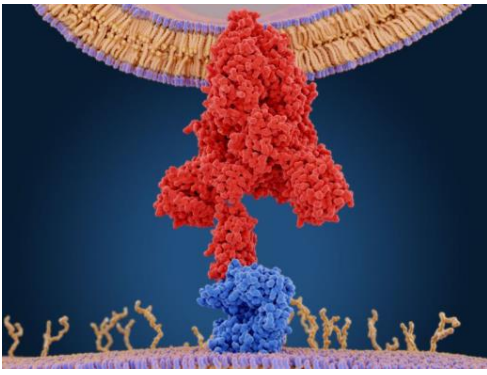
\includegraphics[width=0.65\linewidth]{images/pareja51_01}
\figcaption{Coronavirus Spike Protein and Receptor, Illustration.}

\end{minipage}

\end {flushleft}

Cuando un virus, como el SARS-CoV-2, ingresa al cuerpo humano, este se acopla a las células
del huésped utilizando su estructura proteica externa, su corona. Cuando se produce esta
invasión, el sistema inmunológico reacciona atacando al virus, pero de forma muy lenta.
Conociendo estos hechos, los científicos que diseñan las vacunas buscan crear ``versiones

debilitadas'' de los virus que puedan administrarse a las personas de forma segura y que
permitan a su sistema inmunológico entrenarse en el reconocimiento de los virus y así atacarlos
de forma más eficiente.

\textbf{Microscopio criogénico de electrones}

Una de las herramientas tecnológicas utilizadas para crear el modelo tridimensional del coronavirus es el
microscopio criogénico de electrones, una herramienta que permite ``tomar fotografías'' a una resolución
extremadamente pequeña, a nivel de angstroms. Los avances recientes en tecnología de detectores y
algoritmos de software han permitido la determinación de estructuras biomoleculares con una resolución casi
atómica.

\begin {flushleft}
\noindent\begin{minipage}[c]{\columnwidth}

\centering

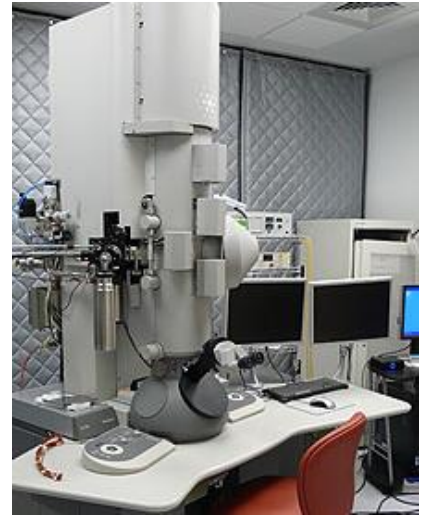
\includegraphics[width=0.65\linewidth]{images/pareja51_02}
\figcaption{Microscopio criogénico de electrones.}

\end{minipage}

\end {flushleft}

Para poder describir la forma tridimensional de un virus mediante el microscopio electrónico, primero se coloca
una muestra del virus en una placa de metal especial, la cual se congela hasta alcanzar aproximadamente los -100 °C.
El microscopio produce como resultado una serie de imágenes bidimensionales que son procesadas por
poderosas computadoras que las combinan para producir la forma final en 3D.

Este proceso fue llevado a cabo por el Doctor Jason McLellan, Profesor Asociado de la Universidad de Austin en Texas, quien,
junto con su equipo de trabajo, desarrolló el modelo tridimensional del SARS-CoV-2 utilizado para la creación las
primeras vacunas contra la COVID-19.

Ahora más que nunca el desarrollo de la tecnología demuestra ser una herramienta de inmenso valor para la supervivencia humana.

Estamos seguros de que la creación y mejora de los dispositivos actuales, junto con el diseño
de avanzados algoritmos de inteligencia artificial representan, ahora y en el futuro, un baluarte
para la humanidad.

\begin {flushleft}
\noindent\begin{minipage}[c]{\columnwidth}
\centering

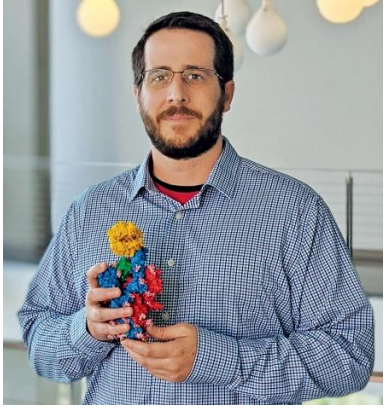
\includegraphics[width=0.65\linewidth]{images/pareja51_03}
\figcaption{Dr. Json McLellan sosteniendo el modelo de la estructura del virus SARS-CoV-2 impreso mediante tecnología de impresión 3D.}

\end{minipage}

\end {flushleft}

\hypertarget{referencias-5}{%
\section{Referencias}\label{referencias-5}}

\begin{itemize}
\item
  {[}1{]} {[}Ryan Cross.{]} {[}\emph{The tiny tweak behind COVID-19 vaccines}{]} Recuperado de: \url{https://bit.ly/3kElV0d}. {[}Último acceso: agosto de 2021{]}.
\item
  {[}2{]} {[}Biology, Integrative. 2021.{]}{[}\emph{Mclellan, Jason - Molecular Biosciences - CNS Directory}{]}.
  Recuperado de: \url{https://bit.ly/3ucAZp7}. {[}Último acceso: agosto de 2021{]}.
\item
  {[}3{]} {[}Del Laboratorio A La Vacuna: Cómo La Tecnología Apoya A Los Fabricantes De Equipo Farmacéutico Para Mantenerse Como Los Mejores De Su Clase"{]}{[}\emph{News Center Latinoamérica}{]}. Recuperado de: \url{https://bit.ly/2XNlVSE}. {[}Último acceso: agosto de 2021{]}.
\item
  {[}4{]} {[}La Tecnología Detrás De Las Vacunas{]}.{[}* Auto-
  mática E Instrumentación - La Revista De La Industria 4.0*{]}. Recuperado de: \url{https://bit.ly/2XUPmTq}. {[}Último acceso: agosto de 2021{]}.
\end{itemize}

\end {multicols}

\medskip

\HRule

\medskip

\hypertarget{pareja58}{%
\chapter{Pandemia del COVID-19 confirma la modernización del ERP a la nube}\label{pareja58}}

\begin{center}
\includegraphics[width=1\linewidth]{images/pareja58_01} \end{center}

\begin {multicols}{2}

\hypertarget{artuxedculo-6}{%
\section{Artículo}\label{artuxedculo-6}}

En el último año pasamos de tener actividades grupales frecuentes (Trabajo, Negocios,
Estudios) a resolver todo de forma remota utilizando una conexión a internet y esta se ha
vuelto vital para nuestro día a día, la razón: El virus COVID-19. Este cambio nos afecta a
todos y nos cambió la forma de hacer las cosas, así como la forma de planificar a futuro.
Enfoquémonos en el mundo empresarial, es muy común que las empresas de mediano
alcance tengan software ERP. ERP son las siglas en inglés de ``planificación de recursos
empresariales'', pero ¿Qué significa ERP? La forma más sencilla de definir ERP es pensar
en todos los procesos centrales necesarios para operar una empresa: Finanzas R.R.H.H.
manufactura, cadena de suministros, servicios, compras y otros. En su nivel más básico el
ERP integra estos procesos en un solo sistema (www.sap.com 2021).

Por lo regular el uso de un ERP en una empresa está acompañado de la implementación de
infraestructura propia para proteger la información, en la mayoría de los casos las empresas
lo prefieren así por temas de seguridad sin embargo son repetidas las veces en las que no
pueden llegar a madurar sus procesos de mantenimiento y el resguardo de la información
porque no tienen la experiencia necesaria, o su giro de negocio no es mantener un data center
con políticas para que la infraestructura esté saludable. Hacerlo es complicado y los costos se
disparan porque aparte de la infraestructura, se necesita recurso con experiencia y esto no es
barato, pero aun así no es imposible y existen empresas en nuestro país que aún han tomado
ese desafío.

Pero en el último año las empresas que tenían su propia infraestructura para sus propios
sistemas ERP se vieron afectadas ya que el acceso a las empresas fue menor, todo se hizo
desde casa y la inversión en sistemas de red privada virtual (vpn) fueron de los costos
cubiertos por las empresas para poder aprovechar su fuerza laboral y no detener sus
operaciones.

Pero todo este escenario está frente a un cambio significativo y es que todas o al menos la
mayoría de software ERP disponible en el mercado y libre, tiene su versión en la nube (por
suscripción) que nos da múltiples ventajas respecto al software ``on premise'' o ``en la
empresa'' algunas de las ventajas a mostrar respecto a estos ERP en la nube, que no son más
que plataformas de software como servicio son las siguientes:

\begin{itemize}
\item
  Acceso remoto: Al estar en la nube para acceder solo se necesita una conexión a
  internet.
\item
  Procesamiento de facturas B2B
\item
  Autoservicio de empleados vía recursos humanos y Blockchain.
\item
  El sistema de contabilidad para el intercambio seguro de datos.
\item
  No se necesita un equipo de TI para realizar tareas de mantenimiento del ERP o
  realizar backups para resguardar la información, el servicio cubre estas necesidades y
  se incluyen en el paquete.
\item
  Reducción de costos e implementaciones más cortas, los sistemas erp on premise
  tienden a tener implementaciones más largas y más costosas que los ERP en la nube.
\end{itemize}

La característica más llamativa de la computación en la nube es sin duda la de poder agregar
suficientes recursos en términos de potencia de procesamiento y memoria lo que hace que el
manejo de grandes volúmenes de datos sea asequible y poder incluso llegar a pensar en la
inclusión de inteligencia artificial cómo algo posible. Contar con un sistema con tales
capacidades logran trascender con el propósito y alcance original de un ERP de ser un
sistema contable, de administración de recursos humanos y cadena de suministros.

Cómo un ejemplo de la evolución del erp en la nube es el sistema SAP S/4HANA
Cloud ERP que Magna International Inc implementó. Ésta decisión logró consolidar hasta
cinco sistemas ERP de la compañía logrando así estandarizar procesos. Estos sistemas
conocidos por sus siglas en inglés SaaS(Software as a Service) están marcando tendencia en
el mercado y es la opción a elegir contra la instalación de servidores físicos (On-premise).

Otro aspecto importante que se ha desatado a causa de la pandemia del COVID-19 es el boom
que han tenido las compras en línea. A consecuencia de esto se ha vuelto esencial contar con
un e-commerce debido a la pérdida de protagonismo que han adquirido los establecimientos
físicos. Esta tendencia facilita la usabilidad integrando al ERP la tienda online y de esta
manera el e-commerce tenga mayor protagonismo como parte de la estrategia del negocio.

Cómo se logra visualizar, la digitalización se ha convertido en una necesidad más demanda
en estos tiempos y las empresas han entendido que contar con herramientas que sean seguras
y efectivas, es crucial para aportar una nueva perspectiva a la planificación y estrategia. Las
soluciones de ERP se han vuelto indispensables para hacer frente a este desafío y así
garantizar la competitividad y sostenibilidad del negocio a largo plazo.

\hypertarget{referencias-6}{%
\section{Referencias}\label{referencias-6}}

\begin{itemize}
\item
  {[}1{]} {[}¿Qué es ERP?{]} {[}\emph{Planificación de recursos empresariales}{]}. Recuperado de: \url{https://bit.ly/3EUhCG5}. {[}Último acceso: agosto de 2021{]}.
\item
  {[}2{]} {[}La importancia y valor de VPN comienzan a aumentar tras el impacto inicial del COVID-19{]}. {[}\emph{El mercado global sufrió importantes variaciones a partir de la pandemia en este 2020}{]}. Recuperado de: \url{https://bit.ly/3EQps3P}. {[}Último acceso: agosto de 2021{]}.
\item
  {[}3{]} {[}La pandemia cambió el mercado del software de gestión: la nueva tendencia{]} {[}\emph{INFOTECHNOLOGY}{]}. Recuperado de: \url{https://bit.ly/3i6nKkL}. {[}Último acceso: agosto de 2021{]}.
\item
  {[}4{]} {[}Las 5 tendencias de ERP más críticas para 2020 y más allá{]} {[}\emph{Guía Esencial: Tendencias y predicciones de TI para el 2020}{]}. Recuperado de: \url{https://bit.ly/3i9GpMM}. {[}Último acceso: agosto de 2021{]}.
\item
  {[}5{]} {[}Conoce las 5 tendencias ERP que marcan el 2021{]} {[}\emph{Marques In ERP}{]}. Recuperado de: \url{https://bit.ly/3m0D1Fd}. {[}Último acceso: agosto de 2021{]}.
\end{itemize}

\end {multicols}

\medskip

\HRule

\medskip

\hypertarget{mendez}{%
\chapter{Hacia la construcción automática de grafos del conocimiento desde fuentes de datos heterogéneas}\label{mendez}}

\begin{center}
\includegraphics[width=1\linewidth]{images/Sergio} \end{center}

\begin {multicols}{2}

\hypertarget{introducciuxf3n-3}{%
\section{Introducción}\label{introducciuxf3n-3}}

Los grafos del conocimiento (Knowledge Graph, KG) se han popularizado en la industria desde que Google introdujo este término al describir su propio KG que opera detrás de su motor de búsqueda. Un KG es una base de conocimiento curada: colección de hechos; el cual incluye entidades que están relacionadas unas a otras a través de enlaces etiquetados y dirigidos (predicados). Tanto las entidades como los predicados están definidos típicamente en una ontología. Una ontología es una especificación explícita de una conceptualización (Gruber, 1993); en términos sencillos, es un modelo de datos que abstrae conceptos e interrelaciones de un dominio de conocimiento específico.

Desde el año pasado, varias ontologías han sido publicadas en la literatura científica (principalmente en los campos de medicina, biología y sociología), las cuales modelan y definen diversos conceptos relacionados con la actual pandemia COVID-19 desde diferentes perspectivas. Asimismo, algunos conjuntos de datos de estudios de COVID-19 han sido publicados en diversos formatos. En un mundo ideal, sería beneficioso el crear de forma automática KGs a partir de estos conjuntos de datos asociados con ontologías específicas. Este artículo presenta una introducción a un proyecto sombrilla en curso que intenta resolver este problema, atacando una amplia variedad de retos técnicos con soluciones en tareas específicas.

\hypertarget{artuxedculo-7}{%
\section{Artículo}\label{artuxedculo-7}}

\textbf{Tubería de artefactos de software para la construcción automática de KGs}

Una tubería de construcción para KGs (KG Construc-
tion Pipeline, KGCP) es un conjunto integrado de artefactos de software que automatizan diversas tareas para construir KGs a partir de fuentes de datos específicas. Dependiendo del dominio y la naturaleza de los datos, un KGCP puede incluir diversas tareas para la extracción, limpieza, y preparación de los datos, seguido de la aplicación de diversas técnicas de procesamiento de lenguaje natural (Natural Language Processing , NLP) para el reconocimiento y enlazamiento de entidades identificadas y encontradas en los datos. En general, las técnicas de NLP son útiles cuando los datos son no estructurados como, por ejemplo, aquellos provenientes de documentos codificados en diversos formatos (PDF, DOCX, PPTX, etc.). El autor de este artículo está trabajando en varios proyectos de investigación relacionados que tienen como objetivo el desarrollo de un KGCP para fuentes de datos no estructuradas. A continuación, se presentará una pequeña introducción de algunos de estos componentes. Todos los recursos (código fuente, documentación relevante, arquitectura, demos, y ejemplos) de este KGCP pueden ser accedidos en el siguiente enlace: \url{https://w3id.org/kgcp/}.

MEL (Metadata Extractor \& Loader: Extractor y cargados de metadatos) (Rodríguez Méndez, 2021) es un artefacto de software que integra de forma liviana varias bibliotecas y paquetes para extraer los metadatos y el contenido textual de diversos archivos (más de 20 formatos diferentes). MEL realiza tareas de preprocesamiento, limpieza de datos y un análisis textual básico del contenido (concordancia de patrones -expresiones regulares- y extracción de palabras clave). Los metadatos y contenido textual extraídos se almacenan en archivos en formato JSON (JavaScript Object Notation : Notación de objetos en JavaScript).

TNNT (The NLP/NER Toolkit: La caja de herramientas de NLP/NER) (Seneviratne, 2021) automatiza la tarea de extracción de entidades nombradas categorizadas desde información no estructurada (archivos en diferentes formatos), utilizando diversas herramientas NLP recientes de última generación y modelos NER. TNNT está integrada con MEL. TNNT integra perfectamente en un solo artefacto de software 9 herramientas NLP y 21 modelos NER de última generación, facilitando el análisis NER para información basada en contenido no estructurado. TNNT puede reconocer 18 categorías diferentes de entidades. Los resultados obtenidos (entidades reconocidas) se utilizan en tareas posteriores en el KGCP para enriquecer el KG a ser generado.

J2RM (JSON-to-RDF Mappings: Mapeos de JSON a RDF) (Rodríguez Méndez, 2020) es una herramienta que procesa mapeos de datos en formato JSON a tripletas RDF (Resource Description Framework : Marco de descripción de recursos) guiadas por la estructura de una ontología OWL2 (OWL2 Web Ontology Language : Lenguaje de ontología para la Web). Los mapeos se definen como ``propiedades de anotación'' asociadas con cada entidad de interés definida en la ontología. Dichos mapeos están dentro de un archivo de ontología por lo que pueden distribuirse y ser compartidos fácilmente para automatizar la creación de grafos RDF. Con J2RM, uno puede trabajar con diferentes estructuras JSON donde todos los mapeos se encuentran embebidos en un archivo específico de ontología. Los mapeos J2RM han sido diseñados como extensiones no estándares a la especificación de JSON-Pointer (apuntadores JSON) con sus propias primitivas que definen transformaciones y operaciones básicas aplicadas a los datos JSON. Los mapeos J2RM operan a nivel de clases y propiedades (de tipos de datos, anotación y objetos) definidos en el archivo de la ontología objetivo.

Otros componentes aún en desarrollo que conforman el ecosistema del mencionado KGCP son: KG-I (Integración de KGs) para automatizar tareas de integración (encontrar entidades equivalentes) en diferentes KGs, y KG-ER (Reconciliación de entidades en KGs) que analiza la estructura de KGs para encontrar el conjunto mínimo de atributos (propiedades de tipos de datos) que puede identificar instancias de clases específicas.

\hypertarget{conclusiones-4}{%
\section{Conclusiones}\label{conclusiones-4}}

Bajo el contexto actual de la pandemia de COVID-19, sería muy útil el construir de forma automática KGs basados en RDF, a partir de conjuntos heterogéneos de datos y ontologías OWL2 relacionadas con este tema que han sido publicados en varios campos científicos. Estos KGs acerca del COVID-19, definirían hechos (datos, entidades y predicados), así como conceptos y sus interrelaciones, los cuales brindarían un modelo semántico con el cual se podrían aplicar algoritmos de aprendizaje automático para descubrir patrones en la información, así como aplicar reglas de inferencia para descubrir nuevo conocimiento. Un conjunto de herramientas integradas que automaticen las tareas de construcción de KGs como el KGCP presentado en este artículo, aceleraría el proceso de análisis y descubrimiento de información que coadyuvaría en diferentes áreas científicas para encontrar soluciones a los retos que actualmente nos presenta la actual pandemia.

\hypertarget{referencias-7}{%
\section{Referencias}\label{referencias-7}}

\begin{itemize}
\item
  {[}1{]} {[}Gruber, Tom{]}. {[}\emph{Toward Principles for the Design of Ontologies Used for Knowledge Sharing. International Journal of Human-Computer Studies. 43 (5--6): 907--928. 1993}{]}.
\item
  {[}3{]} {[}Seneviratne, Sandaru, Sergio J. Rodríguez Méndez, Xuecheng Zhang, Pouya G. Omran, Kerry Taylor, y Armin Haller.{]}{[}\emph{``TNNT: The Named Entity Recognition Toolkit'' (version pre-impresa en arXiv)}{]}. Recuperado de: \url{https://arxiv.org/abs/2108.13700}. {[}Último acceso: 2021{]}.
\item
  {[}4{]} {[}Rodríguez Méndez, Sergio J., Armin Haller, Pouya G. Omran, Jesse Wright, y Kerry Taylor. ``J2RM: an Ontology-based JSON-to-RDF Mapping Tool''{]}{[}\emph{(Conferencia; Proceedings of the ISWC 2020 Demos and Industry Tracks: From Novel Ideas to Industrial Practice - co-located with The 19th International Semantic Web Conference - ISWC 2020). CEUR Workshop Proceedings. Vol. 2721. Pp. 368-373}{]}. Recuperado de: \url{http://ceur-ws.org/Vol-2721/paper593.pdf}. {[}Último acceso: 2021{]}.
\end{itemize}

\end {multicols}

\hypertarget{pareja9}{%
\chapter{Análisis de datos en el descubrimiento de complicaciones en mujeres embarazadas que recibieron la vacuna contra el COVID-19}\label{pareja9}}

\begin{center}
\includegraphics[width=1\linewidth]{images/pareja9_01} \end{center}

\begin {multicols}{2}

\hypertarget{introducciuxf3n-4}{%
\section{Introducción}\label{introducciuxf3n-4}}

Debido a la pandemia de COVID-19 que estamos viviendo, se tuvo la necesidad de investigar y crear una vacuna
para mitigar los efectos en la población y poder sobreponernos a esta situación sanitaria como sociedad. Por esta
razón hemos podido ver distintas vacunas creadas, sobre las cuales algunas personas han tenido dudas por la rápida
fabricación. Es importante mencionar que todas las vacunas que salen al mercado tienen que pasar por ciertas etapas
de estudios para asegurar su eficacia y seguridad.

Las tecnologías actuales ayudan a que muchos procesos se agilicen, uno de estos y que es de gran importancia es el
de recolección, almacenamiento y análisis de datos, ya que son la base para los estudios científicos que generan los
avances en la lucha contra el COVID-19. Las tecnologías de información también son de gran ayuda para evitar la
desinformación y presentar estudios que, con evidencia sólida, puedan informar de la mejor manera.

La vacunación en mujeres embarazadas y en etapa de lactancia, ha generado incertidumbre, sobre los riesgos que
esta pueda tener, ya sea sobre la mujer embarazada o su bebé. Gracias a la recolección de datos de grupos de estudio
y el análisis de datos que se han hecho sobre estas bases de información, se han podido verificar y corroborar ciertas
preocupaciones y descubrir como la vacunación en esta etapa puede resultar beneficiosa para el bebé y que grupos
de expertos recomiendan la vacunación en mujeres embarazadas mayores de 12 años.

\hypertarget{artuxedculo-8}{%
\section{Artículo}\label{artuxedculo-8}}

Actualmente las mujeres embarazadas pueden recibir la vacuna contra el COVID-19. Actualmente no hay evidencia
de que alguna vacuna, incluidas las vacunas de COVID-19, causen problemas de fertilidad. Aún así la información
sobre la seguridad de las vacunas de COVID-19 es limitada. La organización Centers for Disease Control and

Prevention (CDC), cuya misión es trabajar las 24 horas del día, los 7 días de la semana para proteger a Estados
Unidos de las amenazas a la salud, la seguridad y la protección, tanto en el extranjero como en los EE. UU. Diseño
la herramienta V-safe. V-safe es un novedoso programa de vigilancia activa de la seguridad de las vacunas basado
en teléfonos inteligentes para monitorear los síntomas del uso de la vacuna COVID-19 en los Estados Unidos.

Dada la falta de información de datos de seguridad de los ensayos clínicos previos al inicio de la vacunación de la
población en EE. UU. contra el COVID-19 en personas embarazadas. La CDC estableció un protocolo para recopilar
información sobre las personas embarazadas que habían sido expuestas a las vacunas COVID-19 y sus bebés. De ese
modo poder monitorear si desarrollaban algún malestar o si tenían efectos secundarios que pudieran perjudicar al
bebé o a la madre.

La idea es poder generar un lago de datos lo suficientemente amplio que permita obtener conocimiento y guía sobre
la vacunación contra el COVID-19 durante el embarazo y poder proporcionar un método adicional para detectar
eventos adversos que justifiquen una evaluación adicional utilizando los sistemas de bases de datos y seguridad
existentes. La CDC planea utilizar V-safe para monitorear a los participantes no hombre que recibieron vacunas
durante el embarazo o en el periodo de preconcepción (30 días antes del último período menstrual) hasta 14 días
después a través de un registro de mujeres embarazadas. Teniendo como último propósito monitorear las vacunas
COVID-19 durante el embarazo y detectar señales de resultados adversos durante el embarazo y el parto.

La recolección de datos inicia con el proceso de registro de las mujeres embarazadas a través de sus líneas de atención
en call center utilizando la herramienta V-safe. El personal del call center estará capacitado para realizar entrevistas
telefónicas con las participantes embarazadas, que incluyen: confirmación de la identidad de la participante de v-safe y si la persona estaba embarazada en el momento de la vacunación o dentro de los 30 días posteriores a la
vacunación, informando a la gestante sobre el registro de embarazos, incluyendo riesgos, beneficios y alternativas,
solicitando consentimiento para participar en el registro y para la divulgación de registros médicos de los proveedores
de atención médica, y solicitar información específica.

Una vez se hayan obtenido todos los datos se realizará un proceso de ETL para poder garantizar la integridad de los
datos. Ejecutando tareas tales como la eliminación de registros duplicados, eliminación de campos inconsistentes
para asegurar la calidad de los datos.

Los datos registrados del embarazo se analizarán mensualmente como mínimo; los informes incluirán análisis
descriptivos de cualquier resultado adverso en las embarazadas. Específicamente CDC quiere calcular tasas de
muerte fetal (aborto espontáneo y muerte fetal), complicaciones del embarazo (embarazo inducidohipertensión,
diabetes gestacional, preeclam-
psia), resultados adversos del parto (parto prematuro, pequeño para edad gestacional,
bajo peso al nacer, estadías en la unidad de cuidados intensivos neonatales), defectos de nacimiento importantes y
otros resultados de interes. Los resultados deben compararse con promedios nacionales, tasas de referencia
publicadas y estimaciones, vistos en otros sistemas de datos. Después de la recolección de datos y al final del proceso
de ETL los datos recolectados por V-safe serán cargados a un servidor seguro Oracle, para su recopilación,
administración y almacenamiento. Oracle ha donado servicios de TI a cualquier agencia que lleve a cabo actividades
relacionadas con COVID-19.

Los avances en las tecnologías de comunicación, podemos ver como esta llega a más personas en poco tiempo, esto
trae muchos beneficios a la sociedad, pero también existe desinformación que, en temas delicados, como la
vacunación contra el COVID-19, puede resultar contraproducente. El auge de las tecnologías para recolección y
análisis de datos permite que los profesionales en distintas áreas puedan realizar estudios de manera mucho más
rápida y poder informar de manera correcta a toda la sociedad. Esto pasa con el tema si es beneficioso que una mujer
embarazada se vacune, ya que existen ciertos temores que pueden hacer que las personas recomienden no hacerlo.
Estudios realizados por CDC, utilizando los datos registrados en la aplicación de v-safe, que recolectó información
de 153,4000 mujeres embarazadas vacunadas contra el COVID-19, mostraron resultados interesantes y beneficiosos
en pro de la vacunación.

Para agosto de 2021 más de 153 mil mujeres participantes de v-safe, indicaron que las vacunas contra el COVID-19
no provocan ningún problema en las mujeres embarazadas ni en sus bebés. Otro informe a analizo los datos de las
mujeres inscritas en V-safe, que se vacunaron antes de las 20 semanas de embarazo, y no se detectó ningún riesgo
mayor, provocado por la vacuna, de un aborto espontaneo.Las vacunas que se utilizaron para este estudio son
Moderna, Pfizer-BioNTech o jhonson \& Johnson.

Uno de los estudios más importantes que se dieron, es sobre lo que se conoce como inmunidad pasiva,realizado por
American Journal of Obstetrics and Gynecology, esto es indica que la madre pueda pasar los anticuerpos generados
a su bebe durante el periodo de gestación. Estos estudios preliminares indican que con vacunas ARNm, se detectaron
anticuerpos generados por la vacunación en el cordón umbilical, lo que indica que la vacuna durante el embarazo
podría ayudar a proteger a los bebés contra el COVID-19.

La pandemia ha demostrado que muchas de las ramas de la ingeniería de sistemas se pueden aplicar de manera
conjunta para ayudar a la sociedad a solventar dificultades, de manera más rápida a como hubiera sido en otros
tiempos, esto lo podemos ver con la velocidad con la que las vacunas fueron generadas. Una de las tecnologías que
ha ayudado, pero no se habla tanto, es la de análisis de datos, donde por medio de la recolección de grandes cantidades
de información, podemos realizar un proceso de transformación y limpieza, para así tener datos verídicos, y poder
tomar conclusiones a partir de esos datos, esto ayuda a los avances que se han podido dar respecto al conocimiento
de la enfermedad, evitar la desinformación y para la generación de la vacuna contra el COVID-19.

\hypertarget{conclusiones-5}{%
\section{Conclusiones}\label{conclusiones-5}}

\begin{itemize}
\item
  El análisis de datos permite realizar descubrimien-
  tos en los datos de forma más rápida y de forma confiable como se
  haría en procesos manuales, donde se deben tabular y depurar los datos; esto permite encontrar relaciones, causas y
  probabilidades en los datos que muchas veces no son tan perceptibles a simple vista y que pueden brindar un
  conocimiento crucial en la toma de decisiones.
\item
  Los procesos de análisis de datos son importantes para que la sociedad pueda estar informada correctamente, evitando
  el pánico y desinfor- desinfor-
  mación, que puede perjudicar procesos como el de vacunación, haciendo que la enfermedad
  pueda afectar a más personas.
\item
  Las mujeres embarazadas y en periodo de lactancia, son parte de la población que más preocupación generaba al
  momento de vacunarse, ya que no se sabía si podría tener algún efecto contrario a la salud de la persona o del bebé,
  por lo que los estudios realizados ayudan a poder confirmar la seguridad que hay al vacunarse durante el periodo de
  gestación y lactancia.
\end{itemize}

\hypertarget{referencias-8}{%
\section{Referencias}\label{referencias-8}}

\begin{itemize}
\item
  {[}1{]} \href{https://www.cdc.gov/}{GobiernoUSA - Departamento de Salud y Servicios Humanos. 2021}.
  {[}\emph{``Registro de embarazos y vacunación contra el COVID-19 de v-safe.'' Centers for Disease Control and Prevention.}{]}. Recuperado de: \url{https://bit.ly/3ucO9m5}. {[}Último acceso: agosto de 2021{]}.
\item
  {[}2{]} \href{https://portal.ingenieria.usac.edu.gt/}{Wollersheim, Susan. 2020}.(\url{https://www.cdc.gov/}) {[}\emph{``FDA Review of Efficacy and Safety of Pfizer-BioNTech COVID-19 Vaccine Emergency Use Authorization Request.'', Vaccines and Related Biological Products Advisory Committee Meeting.}{]}. Recuperado de: \url{https://bit.ly/3kKZsPk}. {[}Último acceso: agosto de 2021{]}.
\item
  {[}3{]} \href{https://www.researchsquare.com/}{Zauche LH, Wallace B, Smoots AN.}{[}\emph{``Receipt of mRNA COVID-19 vaccines during pregnancy and preconception and risk of self-reported spontaneous abortions, CDC v-safe COVID-19 Vaccine Pregnancy.''}{]}. Recuperado de: \url{https://bit.ly/39Fbza9}. {[}Último acceso: agosto de 2021{]}.
\item
  {[}4{]} \href{https://espanol.cdc.gov/}{GobiernoUSA - Departamento de Salud y Servicios Humanos. 2021.}{[}\emph{``Vacunas contra el COVID-19 durante el embarazo y el periodo de lactancia'' Centers for Disease Control and Prevention. }{]}. Recuperado de: \url{https://bit.ly/3AFg5RT}. {[}Último acceso: agosto de 2021{]}.
\end{itemize}

\end {multicols}

\medskip

\HRule

\medskip

\hypertarget{pareja34}{%
\chapter{El aprendizaje síncrono y la tecnología.}\label{pareja34}}

\begin{center}
\includegraphics[width=1\linewidth]{images/pareja34_01} \end{center}

\begin {multicols}{2}

\hypertarget{introducciuxf3n-5}{%
\section{Introducción}\label{introducciuxf3n-5}}

El mundo está en un constante cambio y de la misma manera lo están las formas de
aprendizaje en diferentes grados académicos, desde el preescolar hasta los cursos universitarios,
y esto se ve aun mas impactado por la actual pandemia que se vive debido al virus COVID-19 y
sus distintas variantes, por lo que tecnologías y formas pedagógicas en desarrollo han tenido que
madurar de una manera exponencial para poder adaptarse a la alta demanda de estudiantes desde
el hogar, un ejemplo son las clases en línea o los cursos libres abiertos en línea, como los que
ofrecen plataformas como Platzi o Coursera.

No solamente los alumnos sufren este impacto, los catedráticos también toman un rol
importante en este cambio al modificar sus formas de enseñar a sus alumnos, algunos continúan
utilizando las tradicionales presentaciones por diapositivas hasta el uso de varias herramientas
como talleres, pizarrones digitales, grupos de trabajo entre otros.

\hypertarget{artuxedculo-9}{%
\section{Artículo}\label{artuxedculo-9}}

El efecto de la pandemia en la pedagogía y la implementación de la tecnología como resultado:
Al inicio del año 2020 se dio un estado de pandemia, este comenzó en China y a finales
de marzo se extendió a todo el mundo, esto provocó el cierre de todas las instituciones
educativas y la pausa total del ciclo escolar en todo el mundo. En esta pausa los catedráticos
comenzaron a dar uso de sus currículos en el apartado ``Conocimiento para el manejo de clases
en línea'' y la transición de clases presenciales tomo curso, comenzando en la busca de
metodologías de enseñanza virtual, estas siendo asíncronas o síncronas.

Las asíncronas siendo las interacciones que se dan entre el catedrático y los estudiantes,
pero no ocurren al mismo tiempo, son tales como practicas asignadas, tareas de ensayos a
entregar y video tutorías hechas para un curso en específico. Y las síncronas que son las más
tradiciones ya que son la interacción entre el catedrático y los estudiantes al mismo tiempo, como
se da en un salón de clase, reunión de estudio o discusión de grupo. Ambos tipos de aprendizaje
son necesarios desde antes de la pandemia, la forma correcta de aplicarlos es la mencionada por
Cathy Lewin: ``Tener elementos asíncronos y combinarlos con actividades síncronas''.

La aplicación de la tecnología a la enseñanza asíncrona es fácil, ya que esta existía desde
hace mucho tiempo, los cursos en línea, videos de YouTube explicando algún Framework,
entregables de proyectos, entre muchos otros ejemplos que se implementaban. El problema se
encuentra en la enseñanza síncrona y su fusión con la tecnología.

\spacethreemilis

\hypertarget{la-aplicaciuxf3n-de-la-tecnologuxeda-en-la-enseuxf1anza-suxedncrona}{%
\subsection{\texorpdfstring{\emph{La aplicación de la tecnología en la enseñanza síncrona:}}{La aplicación de la tecnología en la enseñanza síncrona:}}\label{la-aplicaciuxf3n-de-la-tecnologuxeda-en-la-enseuxf1anza-suxedncrona}}

Se ha utilizado la tecnología para la enseñanza síncrona desde hace varios años tanto
como la enseñanza asíncrona, esta se da en algo tan simple como una clase virtual en la que se
encuentra el catedrático dando clase a sus estudiantes, claro esto es en su forma más simple,
antes de pensar en clases virtuales debemos ver la tecnología utilizada en las clases normales.

Al utilizar tecnología se pueden encontrar varios beneficios en el ámbito educativo,
tomemos por ejemplo un pizarrón inteligente que permite un aprendizaje más interactivo y
dinámico por su facilidad de manejar, adaptabilidad al tema enseñado y varias otras
características que varían dependiendo del pizarrón inteligente, este medio tecnológico mejoro la
enseñanza síncrona tanto para el catedrático como para los estudiantes.

Otro medio es la impresión 3D, clases de arquitectura se han vuelta más dinámicas para
los estudiantes y fáciles de enseñar para los catedráticos gracias a la impresión 3D, ya que los
modelos que antes solo se podían ver en imágenes son recreados con precisión milimétrica y con
esto su examinación puede ser real y no solo teórica.

Estos son ejemplo de enseñanza síncrona utilizando tecnología en clases presenciales,
pero la tecnología en las clases síncronas virtuales no parece pasar de conectarse en una sala a la
hora de una clase. Estadísticas muestran que el interés de los estudiantes por un curso decae al
recibirlo de forma virtual, enseñar por medio de una sala puede ser el método más alcanzable
para todos, pero no es el más eficiente para dar resultados en los estudiantes. Se debe llegar a
otra forma de aplicar la enseñanza síncrona a los estudiantes

Ya existen varios métodos de enseñanza síncrona que utilizan tecnología, el más común y
que está en tomando fuerza en su campo es la realidad virtual. Desde 1987 se empezó a utilizar
la realidad virtual, esta al pasar de los años no solo ha llegado a evolucionar, sino que también se
ha vuelto más accesible. En el 2016 se empezó a utilizar el dispositivo celular para simular la
realidad virtual haciendo uso de su giroscopio interno puede adaptar la visión de una persona y
simularla en las posiciones que el escenario desee.

En el 2020 el proyecto de Microsoft llamado ``Microsoft HoloLens'' salió al mercado
fusionando la realidad virtual con la realidad aumentada, en pocas palabras no solo se utilizarán
para simular la presencia del usuario en un lugar, sino que también simularán la presencia de un
objeto en donde se encuentre el usuario. Esto lo podemos ver parecido a utilizar una impresora
3D para mostrar una maqueta, pero ahora por medio de simulación podremos ver la maqueta en
nuestra propia sala de estar.

Estos son los métodos en los cuales la tecnología puede llegar a ayudar en la educación
síncrona, se exige que los estudiantes tengan una computadora, pero se puede crear un visor de
realidad virtual con un celular inteligente, esto apoyara a la educación síncrona y suplementara
su necesidad en estos tiempos. Los estudiantes necesitan las interacciones que se dan en clases
presenciales para desarrollar su aprendizaje, estamos usando tecnología, pero no debemos
limitarnos a imples video llamadas para solventar el problema más grande que se presenta.

\hypertarget{referencias-9}{%
\section{Referencias}\label{referencias-9}}

\begin{itemize}
\item
  {[}1{]} \href{https://www.tandfonline.com/}{Christine Greenhow, Cathy Lewin \& K. Bret Staudt Willet}. {[}\emph{``The educational response to Covid-19 across two countries''}{]}. Recuperado de: \url{https://bit.ly/3kGwqjJ}. {[}Último acceso: agosto de 2021{]}.
\item
  {[}2{]} \href{https://www.tandfonline.com/}{Anne Yates, Louise Starkey \& Florian Flueggen}. {[}\emph{``High school students' experience of online learning during Covid-19: the influence of technology and pedaggogy''}{]}. Recuperado de: \url{https://bit.ly/3CLXAfe}. {[}Último acceso: agosto de 2021{]}.
\item
  {[}3{]} \href{https://rockcontent.com/}{Redator Rock Content.}{[}\emph{``Tecnologia en la educacion: recursos innovadores para mejorar la calidad educativa''}{]}. Recuperado de: \url{https://bit.ly/3kKvniU}. {[}Último acceso: agosto de 2021{]}.
\end{itemize}

\end {multicols}

\medskip

\HRule

\medskip

\hypertarget{pareja70}{%
\chapter{Como la centralización de información puede salvar vidas guatemaltecas: Una vista al sistema de datos poblacional de Estonia, el país más digitalizado del mundo}\label{pareja70}}

\begin{center}
\includegraphics[width=1\linewidth]{images/pareja70_01} \end{center}

\begin {multicols}{2}

La pandemia del coronavirus SARS-CoV-2 ha sido un terrible recordatorio de lo frágil que puede
ser la humanidad y su organización ante dificultades que la amenazan como especie. En estos
momentos es cuando más resalta la necesidad de tener sistemas de salud eficientes y de gran
alcance que puedan proveer de asistencia a toda la población, entre estos grandes retos está los
sistemas de vacunación.

La logística y trabajo detrás de la distribución de las vacunas ha representado todo un desafío;
estos nos han llevado a replantear las existentes medidas y sistemas los cuales no se han dado a
abasto. El poder reemplazarlos con sistemas que cuenten con el apoyo de la tecnología como
ente organizador que coordine de una manera armoniosa el transporte de medicamentos, el
registro de vacunas y de personas vacunadas, el orden geográfico y temporal de administración
de las vacunas y del control de los efectos de la misma son ahora la prioridad para poder llevar
esta situación y las venideras.

Guatemala cuenta con un portal de registro de vacunas donde las personas pueden concertar una
cita especificando la fecha y el lugar deseados para la vacuna1, lo que da una imagen positiva al
pensar en un modelo automatizado efectivo en el registro, pero en realidad describe un escenario
completamente diferente: la página usualmente no notifica a una persona vía SMS que el registro
se ha programado con éxito, por lo que el Ministerio de Salud Pública y Asistencia Social del
Gobierno de Guatemala ofrece la posibilidad de consultar en el portal de registro de vacunas,
perjudicando así la automatización del proceso en cuestión.

Estos factores entre otros han hecho que la logística detrás de la vacunación sea ineficiente,
acercando a la población al riesgo de contagio con complicaciones. Por su parte, Estonia ha
manejado la pandemia con bastante facilidad y todo gracias al manejo de sus datos.

Estonia, un pequeño país del norte de europa de poco más de un millón de personas, ha apostado
a lo largo de las últimas décadas por sistematizar, digitalizar y centralizar su información, lo cual
le ha permitido tener un control preciso del ritmo de vacunación de su población dejando un
precedente más de cómo la digitalización y la sistematización de procesos no solo hace las cosas
funcionar, si no las hace más fáciles para todos. Este país ha sobrevivido exitosamente a la
pandemia en gran parte por su modelo de centralización de información poblacional, materia en
la que Guatemala fracasa en gran manera.

En este artículo profundizaremos acerca de cómo el modelo Estoniano ha permitido salvar vidas
con su agilidad en la logística detrás de la vacunación y en cómo deberíamos tomarlos de
ejemplo para adoptar sus estrategias en Guatemala.

\spacethreemilis
\spacethreemilis

\textbf{Todo en un mismo lugar}

Estonia ha pasado a la historia como el primer país en realizar elecciones con voto virtual de la
historia; pionero en la cultura de la digitalización como estrategia gubernamental es el primer en
hacer el internet como un derecho social para sus ciudadanos. Este país ha apostado por la
burocracia cero haciendo que los procesos como pagar impuestos, abrir una empresa o
divorciarse sean digitales disminuyendo los seres humanos en el proceso y los tiempos
necesarios para estas tareas.

Para lograr esto fueron necesarios una serie de cambios estructurales en el gobierno, empezando
por la centralización de información. Los datos de los ciudadanos se encuentran encapsulados en
un solo software que permite agilidad y practicidad en la manipulación de información para toma
de decisiones y para disminuir tiempos4, toda una ventaja para enfrentarse al COVID-19. Con
este sistema permitieron la localización rápida de casos de contagio y el control de los mismos, a
su vez permitieron un despliegue de sistemas de vacunación igualmente rápidos y efectivos que
lograron aplacar la pandemia en su territorio de forma controlada.

\spacethreemilis

\textbf{Sin burocracia, con transparencia}

Estonia se ha caracterizado por ser un ejemplo internacional de transparencia y poca burocracia5
en sus labores gubernamentales. Estas características le han permitido al país afrontar las crisis
con respuesta coherente y rápida mejorando así la calidad de vida de sus ciudadanos. Con la
pandemia del COVID-19 se mostrado la importancia de la transparencia ya que cuestiones como
la compra de medicamentos e insumos países como Guatemala han mostrado poca eficacia y
duda en si en verdad las adquisiciones se están realizando; estas cuestiones de confianza de los
ciudadanos a la administración de su gobierno es fundamental para que los eventos difíciles
como las epidemias sean mejor llevadas, cuestión en la que Guatemala fracasa.

\hypertarget{conclusiones-6}{%
\section{Conclusiones}\label{conclusiones-6}}

\begin{itemize}
\tightlist
\item
  Las grandes crisis se afrontan con herramientas y con planificación. Cuando un país es deficiente
  en múltiples áreas estas relucen más cuando los problemas aparecen y Guatemala es un claro
  ejemplo de esto; la desorganización, la falta de transparencia, el caos, la desinformación y la
  escasez son uno de los muchos resultados de tener una pobre administración con múltiples
  deficiencias. Países avanzados como Estonia no lo son solo por su riqueza, sino por su educación
  y preparación; estos países han sabido sobrellevar de mejor manera la pandemia por sus políticas
  ágiles y administración eficiente. Si algo debemos imitar de estos países es su capacidad para
  afrontar los problemas y la gran capacidad de decisión de sus líderes, cuestiones que hoy más
  que nunca hacen falta en la tierra de la eterna primavera.
\end{itemize}

\hypertarget{referencias-10}{%
\section{Referencias}\label{referencias-10}}

\begin{itemize}
\item
  {[}1{]} \href{https://prensa.gob.gt/}{Secretaria de Comunicación Social de la Presidencia}. {[}\emph{``Dudas frecuentes en el proceso de registro y vacunación COVID 2021''. Comunicado. En título ``Registro'' (Pregunta 10)}{]}. Recuperado de: \url{https://bit.ly/3obsgmc}. {[}Último acceso: agosto de 2021{]}.
\item
  {[}2{]} \href{https://elpais.com/}{Collera Virginia}. {[}\emph{``Estonia, primer país digital del mundo''}{]}. Recuperado de: \url{https://bit.ly/3ucQm0R}. {[}Último acceso: agosto de 2021{]}.
\item
  {[}3{]} \href{https://www.valitsus.ee/}{Creative Hub Tallinn.}{[}\emph{``Prime Minister Ratas: E-governance has improved transparency of decision-making in the Eastern Partnership countries''}{]}. Recuperado de: \url{https://bit.ly/3zL5dkf}. {[}Último acceso: agosto de 2021{]}.
\end{itemize}

\end {multicols}

\medskip

\HRule

\medskip

\hypertarget{vivas}{%
\chapter{Población de Guatemala durante la vacunación}\label{vivas}}

\begin{center}
\includegraphics[width=1\linewidth]{images/Vivas} \end{center}

\begin {multicols}{2}

Es Pediatra, egresado de la Universidad de San Carlos de Guatemala, tiene un posgrado en
el hospital general San Juan de Dios, ha sido jefe de servicio de una sala de pediatría durante
15 años. Su labor docente cuenta con una trayectoria de 12 años de ser profesor titular de
farmacología de la Facultad de Medicina de la Universidad de San Carlos de Guatemala y al
mismo tiempo tiene 6 años de ser profesor de pregrado de pediatría en el Instituto
Guatemalteco de Seguridad Social.

Su desempeño privado se ha desarrollado como médico titular del Sanatorio el Pilar, afiliado
a varios hospitales privados del Centro Médico La Esperanza.

\textbf{¿Cuál es el crecimiento de contagio de COVID 19 en niños actualmente en Guatemala, existe algún estudio?}

En lo particular, en la clínica con mi socia con la que ejercemos la práctica privada se ha
tenido de 40 a 45 casos, hemos tratado de filtrar de alguna manera la clínica para no ver
afectados a otros pacientes porque hacemos mucho cuidado de niño sano, entonces tratamos
de hacer una breve llamada a la hora de la cita para ver si hay algún síntoma respiratorio
interrogar a la familia si han estado en contacto con alguien contagiado aunque yo diría que
de marzo del año pasado a marzo de este año era un poco más sencillo que la gente tuviera
idea si había estado en contacto o no, de abril para acá el contagio ha sido muy rápido.

\textbf{¿Cuáles serían los síntomas o se ha visto algún patrón que se presente en todos los casos enfocado a los niños?}

Yo le diría que en pediatría es un poco menos clásico la manifestación del cuadro clínico que
en el adulto, hemos tenido los familiares de los niños que se han infectado que han tenido
digamos que la triada anticlásica que lo hace a uno sospechar, congestión nasal, con pérdida
del olfato, fiebre , dolor de cabeza y dolor de garganta al principio, luego de unos días
empiezan con tos dificultad para respirar y la mayoría de adultos como niños después de 8 o
10 días empieza a disminuir el cuadro, lamentablemente hay mucho que estudiar todavía se
han visto algunas respuestas inflamatorias después del octavo al décimo día donde empiezan
a aparecer algunos otros marcadores bio químicos en nuestro cuerpo que indican que la
infección está acelerada y va en aumento y a veces el virus puede que ya no esté, sin embargo
la respuesta inflamatoria continúa al igual en niños aunque afortunadamente tanto
estadísticas mundiales en los últimos artículos que hemos revisado, ayer precisamente salió
un artículo con varias revisiones bibliográficas de Medicina basada en evidencia de
Latinoamérica, Europa y Estados Unidos, lo presentó la asociación pediátrica a todos los
pediatras asociados y donde se hacía ver algunos cuadros de niños con comorbilidades en
unos niños obesos, niños con algún patrón que ya de algún problema respiratorio crónico,
cardíaco o alguna enfermedad genética que nos hacía predisponer a presentar complicaciones
mayores al igual que la mayoría de los adultos por arriba de los 60 años no se sabe todavía
qué es lo que desencadena una respuesta inflamatoria en algunos si y otros no.

\textbf{¿De los niños que usted ha atendido que presentan un cuadro de COVID 19, como han evolucionado los niños, se han recuperado completa-
mente?}

En algunos casos sí, he sabido de otros colegas que han tenido chicos que sí se han
complicado pulmonarmente, que han hecho un proceso cardiaco también, en el caso de unos
chicos en particular que le contaba al principio afortunadamente ambos están bien, la nena
estuvo como una semana en el seguro social estuvo en el intensivo con un tratamiento
antinflamatorio, con anticoagulantes y inmunoglobulinas que es una sustancia que utilizamos
para anticuerpos circulantes y lograr disminuir la respuesta inflamatoria sistémica, se llama
síndrome inflamatorio sistémico por las siglas en inglés, donde el paciente puede tener mucho
daño en muchos vasos hace una vasculitis, es una inflamación en todos los vasos, entonces
el niño puede tener una conjuntivitis sin secreción, se ven ganglios inflamados, se ven
lesiones en las manos y en las plantas de los pies que son vasitos que se han cerrado y al final
eso puede aumentar el proceso de coagulación, formar un trombo y tapar las arterias más
pequeñas independientemente de la edad son las cerebrales y coronarias, entonces hay niños
que tienen una enfermedad parecida a la descrita por el Doctor Kawasaki hace muchos años
que es una respuesta inflamatoria sistémica o muy parecido al síndrome de Kawasaki que
puede provocar incluso una neurisma al corazón y en algunos niños puede ser de mortal sino
se trata o no se trata a tiempo.

\textbf{¿Cómo visualiza la vacunación en Guatemala? ¿considera usted que es algo a largo plazo?}

Bueno la podríamos enfocar desde 2 puntos de vista, uno es la realidad que nos acople a
nosotros aquí en nuestro país y el otro es el que quisiéramos tener, a nivel mundial se ha
visto que el efecto rebaño, se llama de esa manera porque en efecto, mientras más gente este
vacunada disminuye la posibilidad de contagio, no es que el paciente vacunado no vaya a
contagiar, si no que la carga viral es mucho menor y la posibilidad de presentar un cuadro
grave si es bajísimo comparado a un paciente no vacunado, en Europa, Estados Unidos se ha
visto empezaron por ejemplo el ciclo escolar ahora y están yendo los niños a las escuelas ya
de manera normal, algunos estados están a favor o en contra del uso de la mascarilla sí todos
los profesores están vacunados y los niños están vacunados. El virus es un parasito celular
indispensable eso quiere decir que el virus necesita células para seguirse replicando si no
encuentra las células pero aunque usted tosa se limpia el área y no encuentras células se
muere porque necesita alguien que le sirva de hospedero para seguirse replicando, esa es la
idea de mantener la mascarilla de mantener el distanciamiento social que el virus de la
persona que está infectada no alcance a los demás entonces una buena medida que ha sido
eficaz es el distanciamiento y el uso de la mascarilla, en cuanto a la vacuna propiamente
dicho hay pocos estudios de seguridad en niños y sin embargo Pfizer específicamente con la
tecnología de BioNTech que tiene de ARM mensajero es parte de la ARM del virus que
inyecta a uno, no puede provocar la infección porque tiene como replicarse totalmente en la
copia del ADN, existen otras que solo una espiga, una proteína unida a otro virus más suave
atenuado que está usando AstraZeneca o Jonson por ejemplo, esto acarrea un virus que le
hace la infección a uno más leve pero como no tiene toda la capacidad genética no se puede
replicar en nuestro cuerpo pero si puede tener una respuesta inflamatoria para que el cuerpo
reconozca esa parte de la proteína del virus cuando usted tiene contacto con el virus completo
del cuerpo se recuerda y tiene anticuerpos tiene defensas y entonces la respuesta es menor,
en cuanto a la pediatría pues diríamos que es algo que ilusiona la posibilidad, ya sea con
donativos , independientemente de la gestión del Gobierno.

\textbf{¿Porque algunos tenemos reacción a la vacuna y otros no? ¿cómo es este proceso en nuestro cuerpo?}

Digamos que todas las vacunas que utilizan el antígeno que es una partícula ya sea del virus
o una bacteria al entrar al cuerpo, nuestro cuerpo tiene un sistema humoral y un sistema
celular que reconoce que se le está invadiendo, por lo tanto trata a través de las células,
linfocitos, macrófagos que son nuestra primera línea de defensa de englobar, estudiar el ADN
a veces hacer una copia una réplica y ver cómo por un lado se destruyen porque tenemos
sustancias dentro de las células que lo pueden destruir aunque algunas células algunas
muestras se mueran con el bicho que nos están afectando, la vacuna lo que hace es producir
una respuesta ante la infección qué es lo que pasa que algunos pacientes tiene una respuesta
adecuada u otros no.

\textbf{¿Cuáles considera usted que han sido los aportes de la tecnología en el proceso de vacunación?}

Muchísimo podríamos decir en la tecnología de la comunicación ya que hemos estado más
informados, probablemente si esto hubiera pasado hace unos 10 años ya nos hubiéramos
enterado cuando estuviéramos infectados, en cambio ahora nosotros veíamos las estadísticas
los reportes a nivel mundial, los nuevos infectados ayer en China se está viendo en el mundo
al día siguiente entonces eso ha sido un avance.

Dentro de los avances tecnológicos están las vacunas de RNA mensajero pues hace años no
se pensaba en estudiar esta tecnología es un avance científico que dio un paso gigantesco a
lo que se venía de 10 años de estar estudiando uno que otro virus ahora esta ponencia de las
vacunas con la urgencia que había demostrado un avance gigantesco yo diría que utilizamos
ahora va a tener esta nueva tecnología de pedacitos de copias de ARN en una porción del
ADN de unos virus y bacterias, por ejemplo la vacuna contra la tos y la tosferina la que nos
pusieron a mi generación era una bacteria completa adormecida y nos provocaba una
infección parecida a la que da la tosferina y así quedábamos inmunizados, probablemente a
usted le toco una parte de la pared celular, probablemente a la que ya estamos poniendo ahora
la que se le puso a mi hijo menor ya sólo tiene una parte de la pared celular entonces ya es
imposible que un paciente se infecte con esa parte nada más y el anticuerpo que produce es
efectivísimo entonces con este ejemplo de la vacuna de la tosferina ha ido evolucionando de
acuerdo a los avances de la tecnología y las últimas dos diría de acuerdo a estas dos últimas
de ARN que es una copia de ingeniería genética que se hizo de un antígeno de la superficie
del virus de hepatitis B ósea ya no utilizan el ADN ni parte del ADN sino solo una copia de
un antígeno que lleva una capa de lo que se copió de la proteína del Coronavirus entonces el
antígeno de la superficie del hepatitis B si usted tiene contacto es una enfermedad mortal en
cambio hora desde recién nacidos se puede utilizar esa vacuna con ingeniería genética y el
paciente está protegido de COVID.

\textbf{Doctor cómo visualiza el retorno a la presencialidad, ¿lo recomienda en Guatemala?}

Actualmente por la cantidad de vacunados y con la cantidad tan alta de nuevos contagios, yo
no lo veo prudente, aun en otros países como vimos en la prensa hoy y en las noticias han
abierto las escuelas para muchos lugares, en Guatemala hacen falta muchos recursos, mucha
conciencia social de nuestras autoridades de poder invertir en salud y en los más necesitados.

\textbf{¿Qué efectos positivos y negativos considera que ha traído la educación virtual en la educación de los niños principalmente?}

Nosotros y los que vean esta entrevista somos afortunados, pero es menos del 2\% de la
población nacional, cuántos niños se están rezagando en educación a nivel nacional porque
hay muchas escuelas en el área rural que no tienen acceso a una computadora, escuelas no
digo niños en sus casas y muchos tienen acceso al teléfono y algunos ahí reciben las tareas,
pero es un mínimo de la población.

\textbf{¿Conoce el dato exacto de mortalidad de los niños en hospitales públicos del país?}

desafortunadamente no tengo un dato estadístico certero otro problema es que el Ministerio
de salud tampoco lo tiene no crea que van más avanzados adelante de mi en cuanto a la
información porque la estadística nacional en cuanto a salud es muy pobre, algo hemos
adelantado ahora con la informática, pero estamos muy rezagados, pero afortunadamente yo
me atrevería a decir que el número de niños fallecidos por COVID 19 es muy bajo.

\textbf{Doctor recomendaciones generales para la población de Guatemala, especialmente para la comunidad estudiantil de la Escuela de ingeniería en Ciencias y Sistemas.}

Usar mascarilla cuando estén cerca de otras personas, el lavado de manos que se ha
demostrado científicamente y eficazmente que es una medida que nos protegen de este virus
yo he tenido la fortuna de atender incluso partos y cesáreas de mamás que están contagiadas
en ese momento y con todas las medidas pues aquí me ves a mí salvo no me he contagiado
por que he seguido todas las medidas pero también por el otro lado necesita células y si
nosotros no le damos la nuestras pues no vamos a infectar si nos cuidamos todos podemos
tener un futuro cercano más agradable que podamos compartir, podemos regresar a nuestra
normalidad en un futuro si todos ponemos empeño y cada quien en su pedacito hace bien lo
que le toca yo creo que eso no necesita mayor ciencia ni educación solo necesitan tener un
poco de solidaridad somos un país grande necesitamos los unos a los otros para poder
avanzar

\end {multicols}

\medskip

\HRule

\medskip

\hypertarget{pareja1}{%
\chapter{El impacto de la brecha digital en el acceso a la información de centros de vacunación}\label{pareja1}}

\begin{center}
\includegraphics[width=1\linewidth]{images/pareja1_01} \end{center}

\begin {multicols}{2}

\hypertarget{introducciuxf3n-6}{%
\section{Introducción}\label{introducciuxf3n-6}}

La pandemia del COVID-19 ha dejado en claro la importancia de los medios digitales para
lidiar y progresar como sociedad durante tiempos de crisis; el acceso a internet ha sido clave
para que la población se encuentre informada de la situación actual de la pandemia y del
proceso de inmunización que se está llevando a cabo. En el Plan Nacional de Vacunación
Contra Contra COVID-19 de la República De Guatemala publicado en marzo del 2021, se
detalla el uso de los medios electrónicos para el registro, asignación de citas en centros de
vacunación, seguimiento y emisión de certificados de vacunación.

Si bien el Plan Nacional de Vacunación reconoce la importancia de contar con diferentes
medios para informar a la población sobre la vacunación, con especial énfasis en aquellos
que no tienen acceso a internet o conocimiento del uso de éste, rápidamente ha quedado clara
la ineficiencia del Gobierno para transmitir la información sobre los centros de vacunación
habilitados, por lo que muchas personas se han volcado al uso de páginas y grupos en redes
sociales no oficiales, para poder obtener información sobre los centros de vacunación, los
horarios de atención y el tipo de vacuna que se está aplicando.

El uso de redes sociales y otros medios digitales ha ayudado a la población a poder realizar
su proceso de vacunación de una forma más rápida y eficiente, sin embargo, únicamente la
población con acceso a internet ha sido la que se ha visto beneficiada por estos medios.
Existe un gran porcentaje de la población a la cual la poca facilidad de acceso a internet ha
impedido que puedan informarse correctamente sobre los centros de vacunación habilitados
cerca de su locación, así como de los horarios y disponibilidad de vacunas que se tienen,
demostrando la gran brecha digital que se tiene entre los diferentes sectores de la población
de Guatemala.

\hypertarget{artuxedculo-10}{%
\section{Artículo}\label{artuxedculo-10}}

Vacunas para algunos, información para pocos, vacunación para menos.
Existen situaciones en las que lamentablemente las soluciones a pesar de ser eficientes y estar
realizadas con estándares de calidad que aseguran su funcionamiento, no proporcionan una
solución apropiada para las circunstancias y el entorno en que deben ejecutarse, el cual ha
sido el caso de la comunicación de la información respecto a los centros de vacunación, sus
horarios, fechas y vacunas.

La situación es consecuencia de diversos factores que han desencadenado en dar un lento y
reducido alcance del porcentaje de vacunación. Afortunadamen-
te el porcentaje de
vacunación está aumentando con una tendencia positiva y en crecimiento, en números
significa que aproximadamente solo un 6\% ha logrado completar las dos dosis, sin embargo,
afortunadamente el porcentaje de personas que ha logrado obtener al menos una dosis ha sido
casi el 20\%.

Recientemente el Ministerio de Salud habilitó el portal YoMeVacuno
(\url{https://yomevacuno.gob.gt}) el cual cuenta con información sobre los diferentes Centros de
Vacunación, el tipo de vacuna que aplican y los horarios de atención. Adicional a ello,
muchos guatemaltecos hacen uso de las redes sociales para obtener información de los
centros de vacunación ya que muchas veces estas fuentes resultan ser más fiables que la
información oficial proporcionada.

Los sistemas digitales presentados por el gobierno, si bien cumplen con sus funciones, su
verdadero problema radica en el alcance que posee, puesto que, en Guatemala, hasta el año
pasado, solo el 29\% de la población censada tenía acceso a internet, siendo a su vez
Guatemala el país de América Central con menor crecimiento de población con acceso a
internet durante la pandemia habiendo sido este crecimiento de 11\%, resultando así en un
40\% con acceso a este bien.

A estas diferencias en el acceso y conocimiento de uso de las nuevas tecnologías se denomina
brecha digital. Generalmente se suele distinguir entre primera y segunda brecha digital. La
primera brecha digital hace referencia a la diferencia en el acceso a las nuevas tecnologías.
Por su parte, la segunda brecha digital está relacionada con las habilidades de comprensión
y uso de estas tecnologías por parte de la población que tiene acceso a ellas.

\hypertarget{conclusiones-7}{%
\section{Conclusiones}\label{conclusiones-7}}

(El Gobierno de la República de Guatemala ha proporcionado diferentes fuentes de
información y plataformas para divulgación de datos sobre la vacunación y los
respectivos centros de vacunación, sin embargo, para gran parte de la población, el
acceso a esta información o a información alternativa es casi nula debido a la
desigualdad existente en el acceso a internet.

\begin{itemize}
\item
  La brecha digital existente en el país ha demostrado ser un gran factor bloqueante que ha
  contribuido a entorpecer los esfuerzos para lograr la vacunación de la población.
\item
  Se ha demostrado en épocas de campaña electoral la capacidad de comunicación que se
  posee y la multitud de medios que se es capaz de utilizar, se recomienda realizar esfuerzos
  similares para un tema de salud nacional que afecta a toda la población.
\item
  Se sugiere habilitar en los centros municipales un área de atención donde pueda informarse
  al ciudadano información para que pueda realizar su proceso de vacunación, esta área de
  atención deberá ser promocionada para que la población se entere que cuenta con este
  servicio.
\item
  Considerar el uso de otros medios de comunicación más utilizados localmente, como los
  mensajes SMS por ejemplo
\end{itemize}

\hypertarget{referencias-11}{%
\section{Referencias}\label{referencias-11}}

\begin{itemize}
\item
  {[}1{]} \href{https://www.mspas.gob.gt/}{Ministerio de salud pública y asistencia social, Plan nacional de vacunación contra la covid-19 republica de Guatemala}. {[}\emph{Guatemala, Ministerio de salud pública y asistencia social, 2021}{]}. Recuperado de: \url{https://bit.ly/3ESooMB}. {[}Último acceso: agosto de 2021{]}.
\item
  {[}2{]} \href{https://portal.ingenieria.usac.edu.gt/}{Datos Bancomundial Org}. {[}\emph{``Personas Que Usan Internet (\% De La Población) - Guatemala \textbar{} Data''}{]}. Recuperado de: \url{https://bit.ly/3kFdP7E}. {[}Último acceso: agosto de 2021{]}.
\item
  {[}3{]} {[}Recursos Para Prensa.{]}{[}\emph{"Gobierno De Guate-
  mala Habilita Plataforma Digital Para Acceder A Ubicación De Centros De Vacunación, Horarios Y Vacunas COVID-19 }{]}. Recuperado de: \url{https://bit.ly/2ZE1713}. {[}Último acceso: agosto de 2021{]}.
\item
  {[}4{]} \href{https://www.prensalibre.com/}{Natiana Gándara, Prensa Libre.}{[}\emph{``Guatemala Fue El País Donde Menos Creció El Acceso A Internet En Pandemia''}{]}. Recuperado de: \url{https://bit.ly/3kGwPmg}. {[}Último acceso: agosto de 2021{]}.
\item
  {[}5{]} \href{https://protecciondatos-lopd.com/}{Fernando Tablado, Helena Ramírez. Grupo Atico34.}{[}\emph{``Brecha Digital. Definición, Causas Y Consecuencias \textbar{} Grupo Atico34''}{]}. Recuperado de: \url{https://bit.ly/3ERetaa}. {[}Último acceso: agosto de 2021{]}.
\end{itemize}

\end {multicols}

\medskip

\HRule

\medskip

\hypertarget{pareja30}{%
\chapter{Los Beneficios de la Modelación y Simulación a los Sistemas de Vacunación en Guatemala}\label{pareja30}}

\begin{center}
\includegraphics[width=1\linewidth]{images/pareja30_01} \end{center}

\begin {multicols}{2}

Hace aproximadamente año y medio llegó a Guatemala el COVID-19. Por lo que se tomaron
diferentes medidas de prevención para prevenir la propagación de esta enfermedad y así,
afectar a la menor cantidad de la población guatemalteca. Ya este año 2021, se lograron
desarrollar vacunas para contrarrestar esta enfermedad que atacó a todo el mundo. Y
dependerá de cada país y gobierno la forma en que esta se brindará a la población.

Estas vacunas no serán brindadas como cualquier otra vacuna que se coloca a temprana edad.
Deben de ser suministradas a toda la población, lo que implica la creación de un sistema de
vacunación en el que se involucren colas y registro de personas. Para estos sistemas de colas
existe la modelación y simulación que nos ayuda a prever como se comportaría un sistema.

La modelación y simulación consiste en imitar las operaciones de distintas instalaciones o
procesos de la vida real. Normalmente a las instalaciones y procesos de interés los llamamos
sistemas, y para su estudio realizamos algunas suposiciones sobre como funcionan estos
sistemas. Usualmente estos supuestos tienen forma de un modelo matemático o lógico 1
(Averill y Kelton 2007). En eso consiste la modelación y simulación.

La modelación y simulación cuenta con bastantes ventajas que pueden ayudar en sus distintas
aplicaciones. Entre esas ventajas se encuentran la posibilidad de modificar el modelo de
manera rápida, al ser desarrollado en algún software. También, es más económico mejorar el
sistema vía simulación, esto debido a que podemos simular el sistema para ver el
comportamiento de este y modificar algunos aspectos del modelo que después se pueden
aplicar en la vida real. Además, al simular obtenemos datos exactos sobre como se comporta
nuestro sistema 1 (Averill y Kelton 2007).

Esta tiene distintas aplicacio-
nes en muchas áreas. Por ejemplo, en el área de la construcción
se puede utilizar la simulación para estimar la posible duración de una obra y determinar la
manera en que se van a ir requiriendo y utilizando todos los materiales de la obra. Así
optimizando todo el proceso de obtención de materiales cuando se esté trabajando con la
obra. (Hiriam Esparza, Felipe Martínez y Germán Monroy).

También, dentro del área de modelación y simulación podemos tener casos relacionados con
teoría de colas que pueden servir para cualquier situación que involucre una cola. Ya sea un
banco, el cajero de un restaurante de comida rápida, entre otros. Esta teoría de colas es donde
se pueden encontrar aplicaciones más interesantes de la modelación y simulación. En especial
porque abarca muchos sistemas que utilizamos todos los días.

Estos modelos de teoría de colas cuentan con distintas variables, entre las que podemos
mencionar: la fuente de entrada, que es el conjunto de individuos que pueden llegar al sistema
de servicio; clientes, que son cada individuo que pertenece a la población y requieren del
servicio que brinda el sistema; cola, que es el conjunto de clientes en espera; mecanismo de
servicio, que es el procedimiento por el cual se le da el servicio a los clientes 3
(Ninoska Key).

Actualmente se cuenta con un sistema de vacunación en nuestro país ineficiente por lo que es
necesario implementar y modelar un sistema el cual sea mucho más ordenado, eficiente y
optimizado, realizando un estudio de todos los centros de vacunación actuales y así mismo
analizando los datos de cada uno de ellos, con eso se podrá implementar un modelado de un
sistema cuya finalidad sea aumentar la cantidad de guatemaltecos vacunados, al igual
actualmente se cuenta con un registro de personas y asignación de vacunas ineficiente esto
provocando grandes colas en cada uno de los centros de vacunación así mismo provocándola
aglomeración de público en general, es indispensable modelar un sistema el cual nos permite
un registro de personas eficiente y así mismo contar con un control de asignación para la
adquisición de las diferentes dosis de las vacunas, es de suma importancia analizar los datos
de cada uno de los centros de vacunación así mismo para implementar un buen modelo de
sistema y luego implementar el mismo.

Guatemala se encuentra en una crisis, en los sistemas de salud pública ya no se da abasto con
el personal que tiene, igualmente el control de este sistema es totalmente ineficiente por lo
que es necesario implementar de inmediato un sistema de vacunación el cual sea claro,
conciso y eficiente, dado que si esto no se llegara implementar o no se tomen cartas en el
asunto Guatemala se verá en conflictos y su población estará en altamente en peligro e
indefensa contra la pandemia COVID-19 y sus variantes.

\hypertarget{conclusiones-8}{%
\section{Conclusiones}\label{conclusiones-8}}

\begin{itemize}
\item
  La implementación de un modelado de sistema eficiente, claro y conciso el cual ayude
  a agilizar la vacunación en Guatemala dado que si no Guatemala y su población se
  encontraran en peligro ante la pandemia.
\item
  El funcionamiento de sistemas reales mediante la descripción y análisis de un sistema
  de vacunación
\item
  El análisis de los resultados obtenidos mediante diferentes estudios a través de los
  diferentes modelos de sistemas, estadística y probabilidades.
\item
  La importancia de determinar, modelar, analizar y mejorar el comportamiento de los
  sistemas de procesos reales al generar modelos que se adapten a ellos, implementando
  su conocimiento en el uso de herramientas de simulación.
\end{itemize}

\hypertarget{referencias-12}{%
\section{Referencias}\label{referencias-12}}

\begin{itemize}
\item
  {[}1{]} {[}Averill M.Law y W. David Kelton{]}. {[}\emph{Simulation Modeling \& Analysis, 4ta Edición. McGraw Hill}{]}. {[}Último acceso: agosto de 2021{]}.
\item
  {[}2{]} {[}Hiriam Esparza, Felipe Martínez y Germán Monroy{]}. {[}\emph{Simulacíon: Conceptos y evolucíon. Universidad Autónoma Metropolitana}{]}. {[}Último acceso: agosto de 2021{]}.
\item
  {[}3{]} {[}Ninoska Key. Teoría de Colas.{]}{[}\emph{Universidad Alejandro de Humboldt}{]}. {[}Último acceso: agosto de 2021{]}.
\end{itemize}

\end {multicols}

\medskip

\HRule

\medskip

\hypertarget{pareja38}{%
\chapter{¿Cómo un sistema ERP puede salvar y hacer crecer tu negocio en tiempos de pandemia?}\label{pareja38}}

\begin{center}
\includegraphics[width=1\linewidth]{images/pareja38_01} \end{center}

\begin {multicols}{2}

Seguramente, has escuchado mencionar el término ERP. Si no lo has escuchado, te cuento
más sobre estos sistemas. El nombre proviene de las siglas de las palabras en inglés a
Enterprise Resource Planning y como su mismo nombre indica, es un software dedicado y de
gran alcance en las empresas que permiten llevar un control de los recursos se necesitan para
funcionar. Desde el manejo de inventarios, compras, ventas, flujo de dinero y recursos
humanos.

Con la llegada del Covid el mercado sufrió grandes cambios como disminución de recursos
para la manufactura, hasta reducción en el recurso humano, tanto por enfermedad, como por
restricciones gubernamentales en distintos países. Esto trajo como repercusión que el flujo
completo de recursos con el cual funcionaban las empresas, cambiará por completo.

Sin embargo, empresas que ya utilizaban sistemas de ERP y empresas que invirtieron post
COVID en sistemas ERP han logrado mantener una planificación eficiente a pesar de los
problemas que arrastró con sí el COVID. Es por eso que en este artículo vamos a demostrarte,
porque tu empresa debe considerar la implementación de un ERP, y como este te puede
ayudar como herramienta principal ante las adversidades en este tiempo de pandemia.

Los sistemas ERP están diseñados para reducir costos, mejorar los procesos internos, crecer
la productividad, optimizar los recursos y por supuesto incrementar los ingresos de la
empresa. Estos beneficios son más que esenciales y necesarios para cualquier empresa o
microempresa que quiera mejorar su estado ante esta pandemia. Ahora con la pandemia
acechando.

Otros beneficios que ofrece la implementación de estos sistemas, es la posibilidad de que la
mayoría de trabajos se adapten a la modalidad de ``Home Office'' siendo bastante beneficioso
ya que logra disminuir los riesgos de contagio y aumenta la productividad. Facilita la
comunicación haciendo que el teletrabajo sea totalmente exitoso y que haya una excelente
organización para los proyectos.

Para confirmar la eficacia se mostrará algunos datos verídicos:

\begin{itemize}
\item
  Aproximadamente se puede tener un gasto del 2 por ciento a base de los ingresos.
\item
  Puede llegar a tener un 40\% en reducción en costos, un 38\% de reducción de los
  niveles de inventario y un 35\% de reducción de tiempos.
\item
  Un 40\% de las empresas que implementan un ERP indica que tiene mejoras
  operacionales.
\end{itemize}

No todo es miel sobre hojuelas, los sistemas ERP tiene sus contras, las cuales a continuación
se enlistan algunas:

\begin{itemize}
\item
  La implementación inicial puede llegar a ser caro.
\item
  Los beneficios y ganancias no podrían notarse inmediatamente.
\item
  51\% de las empresas puede llegar a tener una interrupción operacional al implementar
  un ERP.
\item
  Los componentes innecesarios pueden llegar a dejar grandes gastos.
\end{itemize}

A la hora de comenzar la implementación del ERP debes tomar en cuenta lo siguiente:

\begin{enumerate}
\def\labelenumi{\arabic{enumi}.}
\item
  Consulta las distintas áreas de la empresa: Con el surgimiento de la pandemia y los
  retos que implicó la actividad atípica en el área comercial, es importante entender
  como esta cada área de tu empresa. Escucha a tu equipo de trabajo en cada área, la
  experiencia de tu equipo te puede dar una luz de las necesidades de tu empresa.
\item
  Detecta los posibles problemas: ¿Es necesario actualizar la infraestructura TI? ¿Con
  qué sistemas quieres que se integre el ERP? ¿Es posible esa integración? ¿Conlleva
  un esfuerzo de transformación que la empresa puede sobrellevar aún en medio de la
  situación económica generada por la pandemia?
\item
  Define el propósito de la implementación: ¿Se debe a que el negocio necesita
  expandirse dada la diversidad de clientes generada por el covid? ¿El detonante es
  ahorrar costes en los procesos para lograr sobrellevar la pandemia? ¿Cuántas personas
  van a utilizarlo? ¿Qué diferentes roles tendrán los usuarios?, ¿Qué departamentos
  tendrán un uso más intensivo?, etc.
\item
  Escoge la mejor propuesta de ERP para tu empresa: En el mercado existen muchos
  productos ERP por lo que tomar esta decisión es cada vez más difícil. Si tienes a tu
  lado a profesionales en servicios IT, todo resultará más sencillo y el nivel de
  satisfacción será mayor, busca ayuda en el tema y encuentra ejemplos de
  implementaciones en empresas parecidas a la tuya.
\end{enumerate}

Puede que al hacer este ejercicio de evaluación interno llegues a la conclusión de que no es el
momento, o de que la empresa aún no está preparada para asumir el cambio, para iniciar el
camino. No te preocupes. No significa el fin de tu empresa. Pero sí, debe servirte como
llamada de atención. Tómate el tiempo que consideres oportuno, pero no esperes a que los
problemas aparezcan como incidencias graves que finalmente tengas que resolver de manera
urgente, y para los que un ERP sería la solución perfecta.

En conclusión, cuando tu empresa se enfrente a problemas como: descontrol de inventario
que afectan a los pedidos, falta de comunicación entre las diferentes áreas de la organización,
generación de gaps de información y datos inconsistentes, duplicados o erróneos, retrasos en
las respuestas a los clientes, ciclos comerciales excesivamente largos. Es indicador de que
tienes que cambiar internamente.

Y la proliferación de la pandemia orilló a muchísimas empresas a estos problemas, de un día
para otro. Así que ten en cuenta esta información para buscar el cambio lo antes posible. Y
asegurarte que estés preparado para una nueva oleada ya sea de pandemia, o de clientes que
te exijan una administración al máximo nivel dentro de tu organización.

\hypertarget{referencias-13}{%
\section{Referencias}\label{referencias-13}}

\begin{itemize}
\item
  {[}1{]} \href{https://www.ld.co.cr/}{Logical Data}. {[}\emph{¿Puede Un ERP Ayudarme Durante El Coronavirus? - Bog - Logical Data. Logical Data}{]}. Recuperado de: \url{https://bit.ly/2Weo4q2}. {[}Último acceso: agosto de 2021{]}.
\item
  {[}2{]} \href{https://corposuite.com.mx/}{Corposuite}. {[}\emph{``Estadísticas ERP: Tendencias de mercado, datos y analisis este 2021''}{]}. Recuperado de: \url{https://bit.ly/39HGX86}. {[}Último acceso: agosto de 2021{]}.
\item
  {[}3{]} \href{https://datisa.es/}{Datisa ERP}{[}\emph{Recomendaciones para implementar un ERP después del Covid-19s - Datisa ERP}{]}. Recuperado de: \url{https://bit.ly/3kLCuHP}. {[}Último acceso: agosto de 2021{]}.
\end{itemize}

\end {multicols}

\medskip

\HRule

\medskip

\hypertarget{pareja67}{%
\chapter{El análisis de datos para identificar efectos secundarios de las vacunas contra el COVID-19}\label{pareja67}}

\begin{center}
\includegraphics[width=1\linewidth]{images/pareja67_01} \end{center}

\begin {multicols}{2}

\hypertarget{introducciuxf3n-7}{%
\section{Introducción}\label{introducciuxf3n-7}}

En Guatemala, se aplican cuatro diferentes tipos de vacunas (Moderna, Pfizer, AstraZeneca y
Sputnik V) las cuales presentan efectos secundarios muy similares entre sí, pero con algunas
variaciones.

Sin embargo, las vacunas están concebidas para dar inmunidad sin el peligro de contraer la
enfermedad contra la que protegen, logrando salvar millones de vidas, y la vacuna contra la
COVID-19 no es una excepción.
También, como cualquier vacuna, las que protegen contra la COVID-19 pueden causar
efectos secundarios.

Los efectos que suelen presentarse después de la vacunación son de intensidad leve o
moderada, que podrían causarle molestias al realizar sus actividades diarias, pero deberían
desaparecer en unos cuantos días. Además en casos muy poco frecuentes se presentan otros
efectos secundarios más graves.

La identificación certera de de todos los efectos que puede producir una vacuna se encuentran
gracias a los ensayos clínicos, y también al avanzado análisis de datos que nos permite
realizar las ciencias de la computación.

\hypertarget{artuxedculo-11}{%
\section{Artículo}\label{artuxedculo-11}}

\textbf{Inteligencia artificial en monitoreo de efectos adversos por las vacunas}

El regulador de medicamentos de Reino Unido utilizó la inteligencia artificial para examinar
cuidadosa-
mente la alta cantidad de datos de los informes de reacciones adversas a las vacunas
contra el covid-19, debido a la gran escala del plan de vacunación de ese país.

La inteligencia artificial se utilizó como parte de un esquema de tarjetas amarillas de la
Agencia Reguladora de Medicamentos y Productos Sanitarios de Reino Unido (MHRA),
donde los médicos y pacientes pueden reportar efectos secundarios o reacciones negativas.
Después la inteligencia artificial entra en juego evaluando si es necesario actualizar las
medidas de seguridad o alguna regulación para proteger a la población.

La importancia del desarrollo de esta herramienta de inteligencia artificial es fundamental ya
que su ausencia podría representar altos riesgos contra la salud pública porque no permite la
capacidad de identificar futuros problemas de salud o de seguridad en la población. Además,
los reportes sobre los efectos secundarios y reacciones podrían ser alterados debido a la
influencia pública y medios sociales. Un reporte de reacciones adversas a medicamentos no
significa que ocurra un efecto secundario debido a la vacuna, sino que existen posibilidades
que la vacuna pudo causar esa reacción.

Por ende, el tiempo de desarrollo de esta herramienta de inteligencia artificial se redujo al
mínimo, ya que es una necesidad para la salud mundial, las vacunas que hayan sido
previamente analizadas se consideran seguras y eficaces.

Sin embargo, esta herramienta servirá sólo de monitoreo y control, ya que la mayoría de los
efectos adversos fueron encontrados en los ensayos clínicos respectivos antes de su
aprobación, aunque no significa que las vacunas no puedan ocasionar efectos secundarios y
reacciones que no hayan sido detectadas en los ensayos clínicos.

La utilización de estos recursos tecnológicos en el monitoreo de los efectos secundarios de las
vacunas contra el COVID-19 ha logrado un avance significativo en medio de la urgencia de
detener la pandemia, mediante la rápida detección de reacciones peligrosas, asegurando a la
población una vacuna segura y eficaz.

\hypertarget{referencias-14}{%
\section{Referencias}\label{referencias-14}}

\begin{itemize}
\item
  {[}1{]} {[}FDA. 2020. U.S{]}. {[}\emph{Food \& Drug Administration.}{]}. Recuperado de: \url{https://bit.ly/2ZoraJd}. {[}Último acceso: agosto de 2021{]}.
\item
  {[}2{]} \href{https://www.who.int/}{OMS. 2020}. {[}\emph{Organización Mundial de la Salud}{]}. Recuperado de: \url{https://bit.ly/3AKH52t}. {[}Último acceso: agosto de 2021{]}.
\item
  {[}3{]} {[}Gross, Anna.{]}{[}\emph{Financial Times}{]}. Recuperado de: \url{https://on.ft.com/3i9JI6I}. {[}Último acceso: agosto de 2021{]}.
\end{itemize}

\end {multicols}

\medskip

\HRule

\medskip

\bibliography{book.bib,packages.bib}

%%%%\printindex




\includepdf{images/contraportada.pdf}


\end{document}
